\chapter{Evaluation}\label{ch:evaluation}

\section{Reference Implementation}

A reference implementation of \cref{sec:asynchronous} is available on GitHub\footnote{\url{https://github.com/cwru-xlab/sharetrace-akka}}. Actors are implemented using the Akka toolkit\footnote{\url{https://doc.akka.io/docs/akka/2.8.5/typed/index.html}}, which offers high performance for large-scale actor systems. Experimental results indicate that the reference implementation can process contact networks with at least 100 thousand \verticesName and 10 million edges on a single machine, so it is suitable for small-scale and medium-scale experiments. In addition to using the Akka toolkit, several other optimizations are implemented.
\begin{itemize}
  \item To reduce the size of event logs and result files, individual actor identifiers follow zero-based numbering and event records are serialized using the Ion format\footnote{\url{https://amazon-ion.github.io/ion-docs}} with shortened field names.
  \item To reduce memory usage, FastUtil\footnote{\url{https://fastutil.di.unimi.it}} data structures are used, including a specialized integer-based JGraphT\footnote{\url{https://jgrapht.org}} graph implementation \citep{Michail2020}. Also, singletons \citep{Gamma1995}, primitive data types, and reference equality are preferred where feasible and do not impact readability.
  \item To reduce runtime and increase throughput, logging is performed asynchronously with Logback\footnote{\url{https://logback.qos.ch/index.html}} and the LMAX Disruptor\footnote{\url{https://lmax-exchange.github.io/disruptor}}.
\end{itemize}

\Cref{fig:arrow-diagram} shows the dependencies among the application components. Contextualizing this implementation with prior implementations of the driver-monitor-worker (DMW) framework (see \cref{sec:dmw-framework}), \class{RiskPropagation} is the driver, \class{Monitor} is the monitor, and \class{User} is the worker. The key difference between this implementation and previous implementations of the DMW framework is that workers are stateful, which is necessary for decentralization.
\begin{figure}[htbp]
\begin{equation*}
  \class{Main} \rightarrow \class{Runner} \rightarrow \class{RiskPropagation} \rightarrow \class{Monitor} \rightarrow \class{User} \rightarrow \class{Contact}
\end{equation*}
\caption[Arrow diagram of the reference implementation]{Arrow diagram of the reference implementation.}
\label{fig:arrow-diagram}
\end{figure}

\Cref{sec:asynchronous} describes the behavior of a \class{User} and \class{Contact}. In order to evaluate \class{RiskPropagation}, each \class{User} logs the following types of \class{UserEvent}:
\begin{itemize}
  \item \class{ContactEvent}: logged when the \class{User} receives an unexpired \class{ContactMessage}; contains the \class{User} identifier, the \class{Contact} identifier, and the contact time.
  \item \class{ReceiveEvent}: logged when the \class{User} receives an unexpired \class{RiskScoreMessage}; contains the \class{User} identifier, the \class{Contact} identifier, and the \class{RiskScoreMessage}.
  \item \class{UpdateEvent}: logged when the \class{User} updates its exposure score; contains the \class{User} identifier, the previous \class{RiskScoreMessage}, and the current \class{RiskScoreMessage}.
  \item \class{LastEvent}: logged when the \class{User} receives a \class{PostStop} Akka signal\footnote{\url{https://doc.akka.io/docs/akka/current/typed/actor-lifecycle.html\#stopping-actors}} after the \class{Monitor} has stopped; contains the \class{User} identifier and the time of logging the final event, besides \class{LastEvent}; used to detect the end time of message passing.
\end{itemize}
For reachability analysis, a \class{RiskScoreMessage} contains the identifier of the \class{User} that propagated it and the identifier of the \class{User} that first sent it.

The \class{Monitor} is an actor that is responsible for transforming the \class{ContactNetwork} into a collection of \class{User}s and terminating when no \class{UpdateEvent} has occurred for a period of time. The \class{Monitor} logs several types of \class{LifecycleEvent}, ordered according to when they are logged during execution:

\begin{multicols}{2}
\begin{enumerate}
  \item \class{RiskPropagationStart}
  \item \class{CreateUsersStart}
  \item \class{CreateUsersEnd}
  \item \class{SendContactsStart}
  \item \class{SendContactsEnd}
  \item \class{SendRiskScoresStart}
  \item \class{SendRiskScoresEnd}
  \item \class{RiskPropagationEnd}
\end{enumerate}
\end{multicols}

\class{RiskPropagation} logs execution properties, creates an Akka \class{ActorSystem} that creates a \class{Monitor} actor and sends it a \class{RunMessage}, and then waits until the \class{ActorSystem} terminates. Each execution of \class{RiskPropagation} is associated with a unique key that is included in each event record as mapped diagnostic context (MDC)\footnote{\url{https://logback.qos.ch/manual/mdc.html}}.

The \class{Runner} specifies how \class{RiskPropagation} is created and invoked, usually through some combination of statically defined behavior and runtime configuration.

Finally, \class{Main} is the entry point into the application. It is responsible for parsing \class{Context}, \class{Parameters}, and \class{Runner} from configuration and invoking \class{Runner} with \class{Context} and \class{Parameters} as inputs. \class{Context} makes application-wide information accessible, such as the system time and user time\footnote{System time is always the wall-clock time and is included in each logged event record. User time is configurable to either be the wall-clock time or fixed at the reference time. The latter ensures that no \class{RiskScoreMessage} or \class{ContactMessage} expires across executions of \class{RiskPropagation}.}, a pseudorandom number generator, \class{Runner} configuration, and loggers. \class{Parameters}, as the name suggests, is a collection of parameters that modify the behavior of the \class{Monitor}, \class{User}s, and \class{Contact}s.

To analyze the executions of \class{RiskPropagation} that are associated with the same  configuration, \class{EventHandler}s process the execution properties and event logs. For each execution of \class{RiskPropagation}, one or more \class{EventHandler}s process the stream of event records and aggregate state about a particular aspect of the execution. Once the event stream has been processed, an \class{EventHandler} may perform a final aggregation or transformation of its state and persist the result in a \class{Results} instance. The contents of the \class{Results} instance is then stored for further analysis. For example, each experiment in \cref{sec:experimental-design} was associated with multiple configurations. The results of those configurations were aggregated and flattened into a tabular dataset, which was subsequently analyzed and presented in \cref{sec:results}.

The following \class{EventHandler}s were implemented for this work:
\begin{itemize}
  \item \class{Reachability}: aggregates \class{ReceiveEvent}s that involve a distinct sender and receiver to determine the influence set cardinality, source set cardinality, and message reachability of each \class{User}.
  \item \class{Runtimes}: aggregates \class{LifecycleEvent}s and \class{LastEvent}s to determine the runtime of creating \class{User}s, sending \class{ContactMessage}s, sending \class{RiskScoreMessage}s, message passing, and the overall execution of \class{RiskPropagation}. Message-passing runtime is the duration between \class{SendRiskScoresStart} and the latest \class{LastEvent}.
  \item \class{UserEventCounts}: aggregates \class{UserEvent}s to determine the frequency of each type for each \class{User}.
  \item \class{UserUpdates}: aggregates \class{UpdateEvent}s to determine the new exposure score of each \class{User} and the change in value.
\end{itemize}

\section{Experimental Design}\label{sec:experimental-design}

The following experiments were used to evaluate \class{RiskPropagation}.
\begin{enumerate}[ref={Experiment \arabic*}]
  \item How does the send coefficient affect accuracy and efficiency?\label{item:parameters}
  \item Do the distributions of risk scores and contact times affect runtime?\label{item:distributions}
  \item How does the size of the contact network affect runtime?\label{item:topology}
\end{enumerate}

\labelcref{item:parameters} was completed first to determine suitable parameter values for the remaining experiments. \labelcref{item:distributions} was conducted before \labelcref{item:topology} to determine the necessity of evaluating all combinations of data distributions. That is, if the type of data distribution was found to have a statistically nonsignificant effect on the runtime of \class{RiskPropagation}, then the complexity of \labelcref{item:topology} could be meaningfully reduced. \labelcref{item:topology} was conducted to determine if a simple model could be used in practice to estimate the message-passing runtime of \class{RiskPropagation}. While \labelcref{item:distributions} and \labelcref{item:topology} focus on benchmarking the reference implementation, more advanced simulation-based analysis of ShareTrace with COVI-AgentSim \citep{Gupta2020} is the subject of future work.

All experiments utilized the same random graphs: Barabasi-Albert graphs \citep{Barabasi1999}, Erd\H{o}s-R\'{e}nyi $G_{n,m}$ graphs \citep{Erdos1959}, Watts-Strogatz graphs \citep{Watts1998}, and random regular graphs \citep{Kim2003}. These graphs were selected because they are available in the JGraphT library and are parametric, either directly or indirectly, in the size and order of the network. The latter property allowed the effects of the topology to be isolated. While Barabasi-Albert graphs, Erd\H{o}s-R\'{e}nyi $G_{n,m}$ graphs, Watts-Strogatz graphs exhibit aspects of real-world contact networks \citep{Newman2003}, random regular graphs do not.

The following describes the parametrization of each type of contact network. Barabasi-Albert graphs are parametrized by the order $n$, the initial order $n_0$, and the increase in size $m_0$ upon each incremental increase in order. The latter two parameters are determined by solving \cref{eq:Barabasi-Albert-optimization}, where $\fracpart(x)$ is the fractional part of a real number $x$.
\begin{argmini}{n_0, m_0}{\fracpart(m_0)}{\protect\label{eq:Barabasi-Albert-optimization}}{}
  \addConstraint{n_0}{\in \intInterval{1}{n - 1}}
  \addConstraint{m_0}{\in \intInterval{1}{n_0}}
  \addConstraint{m_0}{= \frac{2m - n_0 (n_0 - 1)}{2(n - n_0)}}
\end{argmini}
Erd\H{o}s-R\'{e}nyi graphs are parametrized by the order $n$ and the size $m$. Random regular graphs are parametrized by the order $n$ and, using the degree sum formula, the degree $d = \lfloor 2m / n \rfloor$. Lastly, Watts-Strogatz graphs \citep{Watts1998} are parametrized by the order $n$, the rewiring probability $p$, and the number of nearest neighbors $k = d + (d \bmod 2)$.

\Cref{tab:default-parameters} specifies the default parameter values and seed for pseudorandom number generation. \Cref{tab:experiments} specifies the experiment configurations. All experiments used fixed user time. The following sampling process was used to generate risk scores and contact times. Given the probability density function $f_X$ and the cumulative distribution function $F_X$ of a random variable $X$, sample a value $x \sim f_X$ and evaluate $c \cdot F_X(x)$ for some scalar $c \in \reals$. Risk scores are composite data types, so risk score values and risk score times were sampled independently. Because risk scores are probabilities, $c = 1$ was used to scale the values. When sampling the times of risk scores and contacts, $c = \pScoreExpiry$ and $c = \pContactExpiry$ were used, respectively.

\begin{table}[htbp]
  \centering
  \begin{tabular}{ll}
    \toprule
    Parameter & Default value \\
    \midrule
    Transmission rate & \num{0.8}\\
    Send coefficient & \num{1}\\
    Time buffer & \qty{2}{days}\\
    Risk score expiry & \qty{14}{days}\\
    Contact expiry & \qty{14}{days}\\
    Flush timeout & \qty{3}{seconds}\\
    Idle timeout & \qty{1}{minute}\\
    Seed & \num{12345}\\
    \bottomrule
  \end{tabular}
  \caption[Default parameter values for experiments]{Default parameter values for experiments.}
  \label{tab:default-parameters}
\end{table}

\begin{table}[htbp]
  \centering
%  \renewcommand{\arraystretch}{2}
  \begin{tabular}{lc}
    \toprule
    Network type & Parameters \\
    \midrule
    Barabasi-Albert & $\begin{aligned} n &= \num{5000} \\ n_0 &= \num{21} \\ m_0 &= \num{10} \end{aligned}$\\
    \midrule
    Erd\H{o}s-R\'{e}nyi & $\begin{aligned} n &= \num{5000} \\ m &= \num{50000} \end{aligned}$\\
    \midrule
    Random regular & $\begin{aligned} n &= \num{5000} \\ d &= 20 \end{aligned}$\\
    \midrule
    Watts-Strogatz & $\begin{aligned} n &= \num{5000} \\ p &= \num{0.2} \\ k &= \num{20} \end{aligned}$\\
    \bottomrule
  \end{tabular}
  \caption[]{Experiment 1}
  \label{tab:network-parameters}
\end{table}

\begin{table}[htbp]
  \centering
%  \renewcommand{\arraystretch}{2}
  \begin{tabular}{lc}
    \toprule
    Network type & Parameters \\
    \midrule
    Barabasi-Albert & $\begin{aligned} n &= \num{10000} \\ n_0 &= \num{21} \\ m_0 &= \num{10} \end{aligned}$\\
    \midrule
    Erd\H{o}s-R\'{e}nyi & $\begin{aligned} n &= \num{10000} \\ m &= \num{100000} \end{aligned}$\\
    \midrule
    Random regular & $\begin{aligned} n &= \num{10000} \\ d &= 20 \end{aligned}$\\
    \midrule
    Watts-Strogatz & $\begin{aligned} n &= \num{10000} \\ p &= \num{0.2} \\ k &= \num{20} \end{aligned}$\\
    \bottomrule
  \end{tabular}
  \caption[]{Experiment 2}
  \label{tab:network-parameters}
\end{table}

%\begin{table}[htbp]
%  \centering
%  \scriptsize
%  \begin{tabular}{lccccccccc}
%    \toprule
%    Order (thousands) & \multicolumn{9}{c}{Size (millions)} \\
%    \cmidrule(lr){1} \cmidrule(lr){2-10}
%    & $1$ & $2$ & $3$ & $4$ & $5$ & $6$ & $7$ & $8$ & $9$ & $10$ \\
%    $10$ & $BA(n, m)$ & $BA(n, m)$ & $BA(n, m)$ & $BA(n, m)$ & $BA(n, m)$ & $BA(n, m)$ & $BA(n, m)$ & $BA(n, m)$ & $BA(n, m)$\\
%    \bottomrule
%  \end{tabular}
%  \caption[]{Experiment 3}
%  \label{tab:network-parameters}
%\end{table}

\begin{sidewaystable}[htbp]
  \centering
  \renewcommand{\arraystretch}{2}
  \begin{tabular}{lccc}
    \toprule
    Aspect & \labelcref{item:parameters} & \labelcref{item:distributions} & \labelcref{item:topology} \\
    \midrule
    Order $n$, size $m$ & $\begin{aligned} n &= 5 \cdot 10^3 \\ m &= 5 \cdot 10^4 \end{aligned}$ & $\begin{aligned} n &= 10^4 \\ m &= 10^5 \end{aligned}$ & $\begin{matrix} n \in \setBuilder{10^4x}{x \in \intInterval{1}{10}} \\ \times \\ m \in \setBuilder{10^6x}{x \in \intInterval{1}{10}} \end{matrix}$ \\
    Parameters & $\pSendCoefficient \in \setBuilder{10^{-1}x}{x \in \intInterval{8}{20}}$ & Defaults & Defaults \\
    Distributions & $\{\text{Uniform}, \text{Standard normal}\}^3$ & $\{\text{Uniform}, \text{Standard normal}\}^3$ & Uniform \\
    Repetitions & 5 & 1 burn-in + 5 & 1 burn-in + 5 \\
    Networks & 160 (40 per type) per parameter & \num{160} (40 per type) & \num{2000} (500 per type) \\
    \bottomrule
  \end{tabular}
  \caption[Experiment configurations]{Experiment configurations. See \cref{tab:default-parameters} for default parameter values. The notation $X^k$ is used to denote the $k$-ary Cartesian power of the set $X$. A ``burn-in'' repetition was used for \labelcref{item:distributions} and \labelcref{item:topology} to avoid measuring the impact of Java class loading.}
  \label{tab:experiments}
\end{sidewaystable}

\section{Results}\label{sec:results}

Several Python libraries were utilized in the writing of this section. Data visualizations were created with seaborn \citep{Waskom2021} and Matplotlib \citep{Hunter2007}. Tabular datasets were created and analyzed with Polars \citep{Vink2024}. Pingouin \citep{Vallat2018} was utilized in \cref{sec:parameters-experiment} to compute correlation coefficients. SciPy \citep{Virtanen2020} was used in \cref{sec:runtime-baseline-experiment} to perform hypothesis testing. scikit-learn \citep{Pedregosa20211} was used to train and evaluate the quantile regression models in \cref{sec:runtime-experiment}. Lastly, NumPy \citep{Harris2020} was used to support statistical calculation and data visualization.

\subsection{\labelcref{item:parameters}}\label{sec:parameters-experiment}

As indicated in \cref{tab:experiments}, each repetition was associated with a set of send coefficients, a contact network, and a set of symptom scores. For each repetition, the accuracy of a send coefficient $\pSendCoefficient$ was defined over $D_i$, the set of \emph{nonzero}\footnote{It is unclear whether an individual's exposure score was never updated due to the send coefficient or because the actor did not receive any risk scores that were higher than the individual's symptom score. If an individual's exposure score was never updated for any send coefficient, their differences were not considered for evaluation.} differences between \indexed{i}{individual's} exposure score and symptom score,
\begin{equation*}
  f_i(\pSendCoefficient) = 1 - \max D_i + D_i(\pSendCoefficient),
\end{equation*}
where $D_i(\pSendCoefficient)$ is the difference associated with $\pSendCoefficient$. \Cref{fig:accuracy-percentiles} and \cref{tab:accuracy-percentiles} confirm that a send coefficient of $\pSendCoefficient = 1$ produces perfect accuracy. For $\pSendCoefficient > 1$, accuracy degrades for a relatively small percentage of the population. Intuitively, as the send coefficient increases, it becomes likelier for actors to not propagate risk scores that would otherwise update the exposure score of another actor in the network. 

As noted in \cref{tab:accuracy-percentiles}, it is expected that $\pSendCoefficient < 1$ also provides perfect accuracy, given sufficient time for message passing to complete. Because the executions associated with $\pSendCoefficient < 1$ were suspected to be incomplete, the associated data was omitted from the remainder of this analysis.

\begin{figure}[htbp]
  \centering
  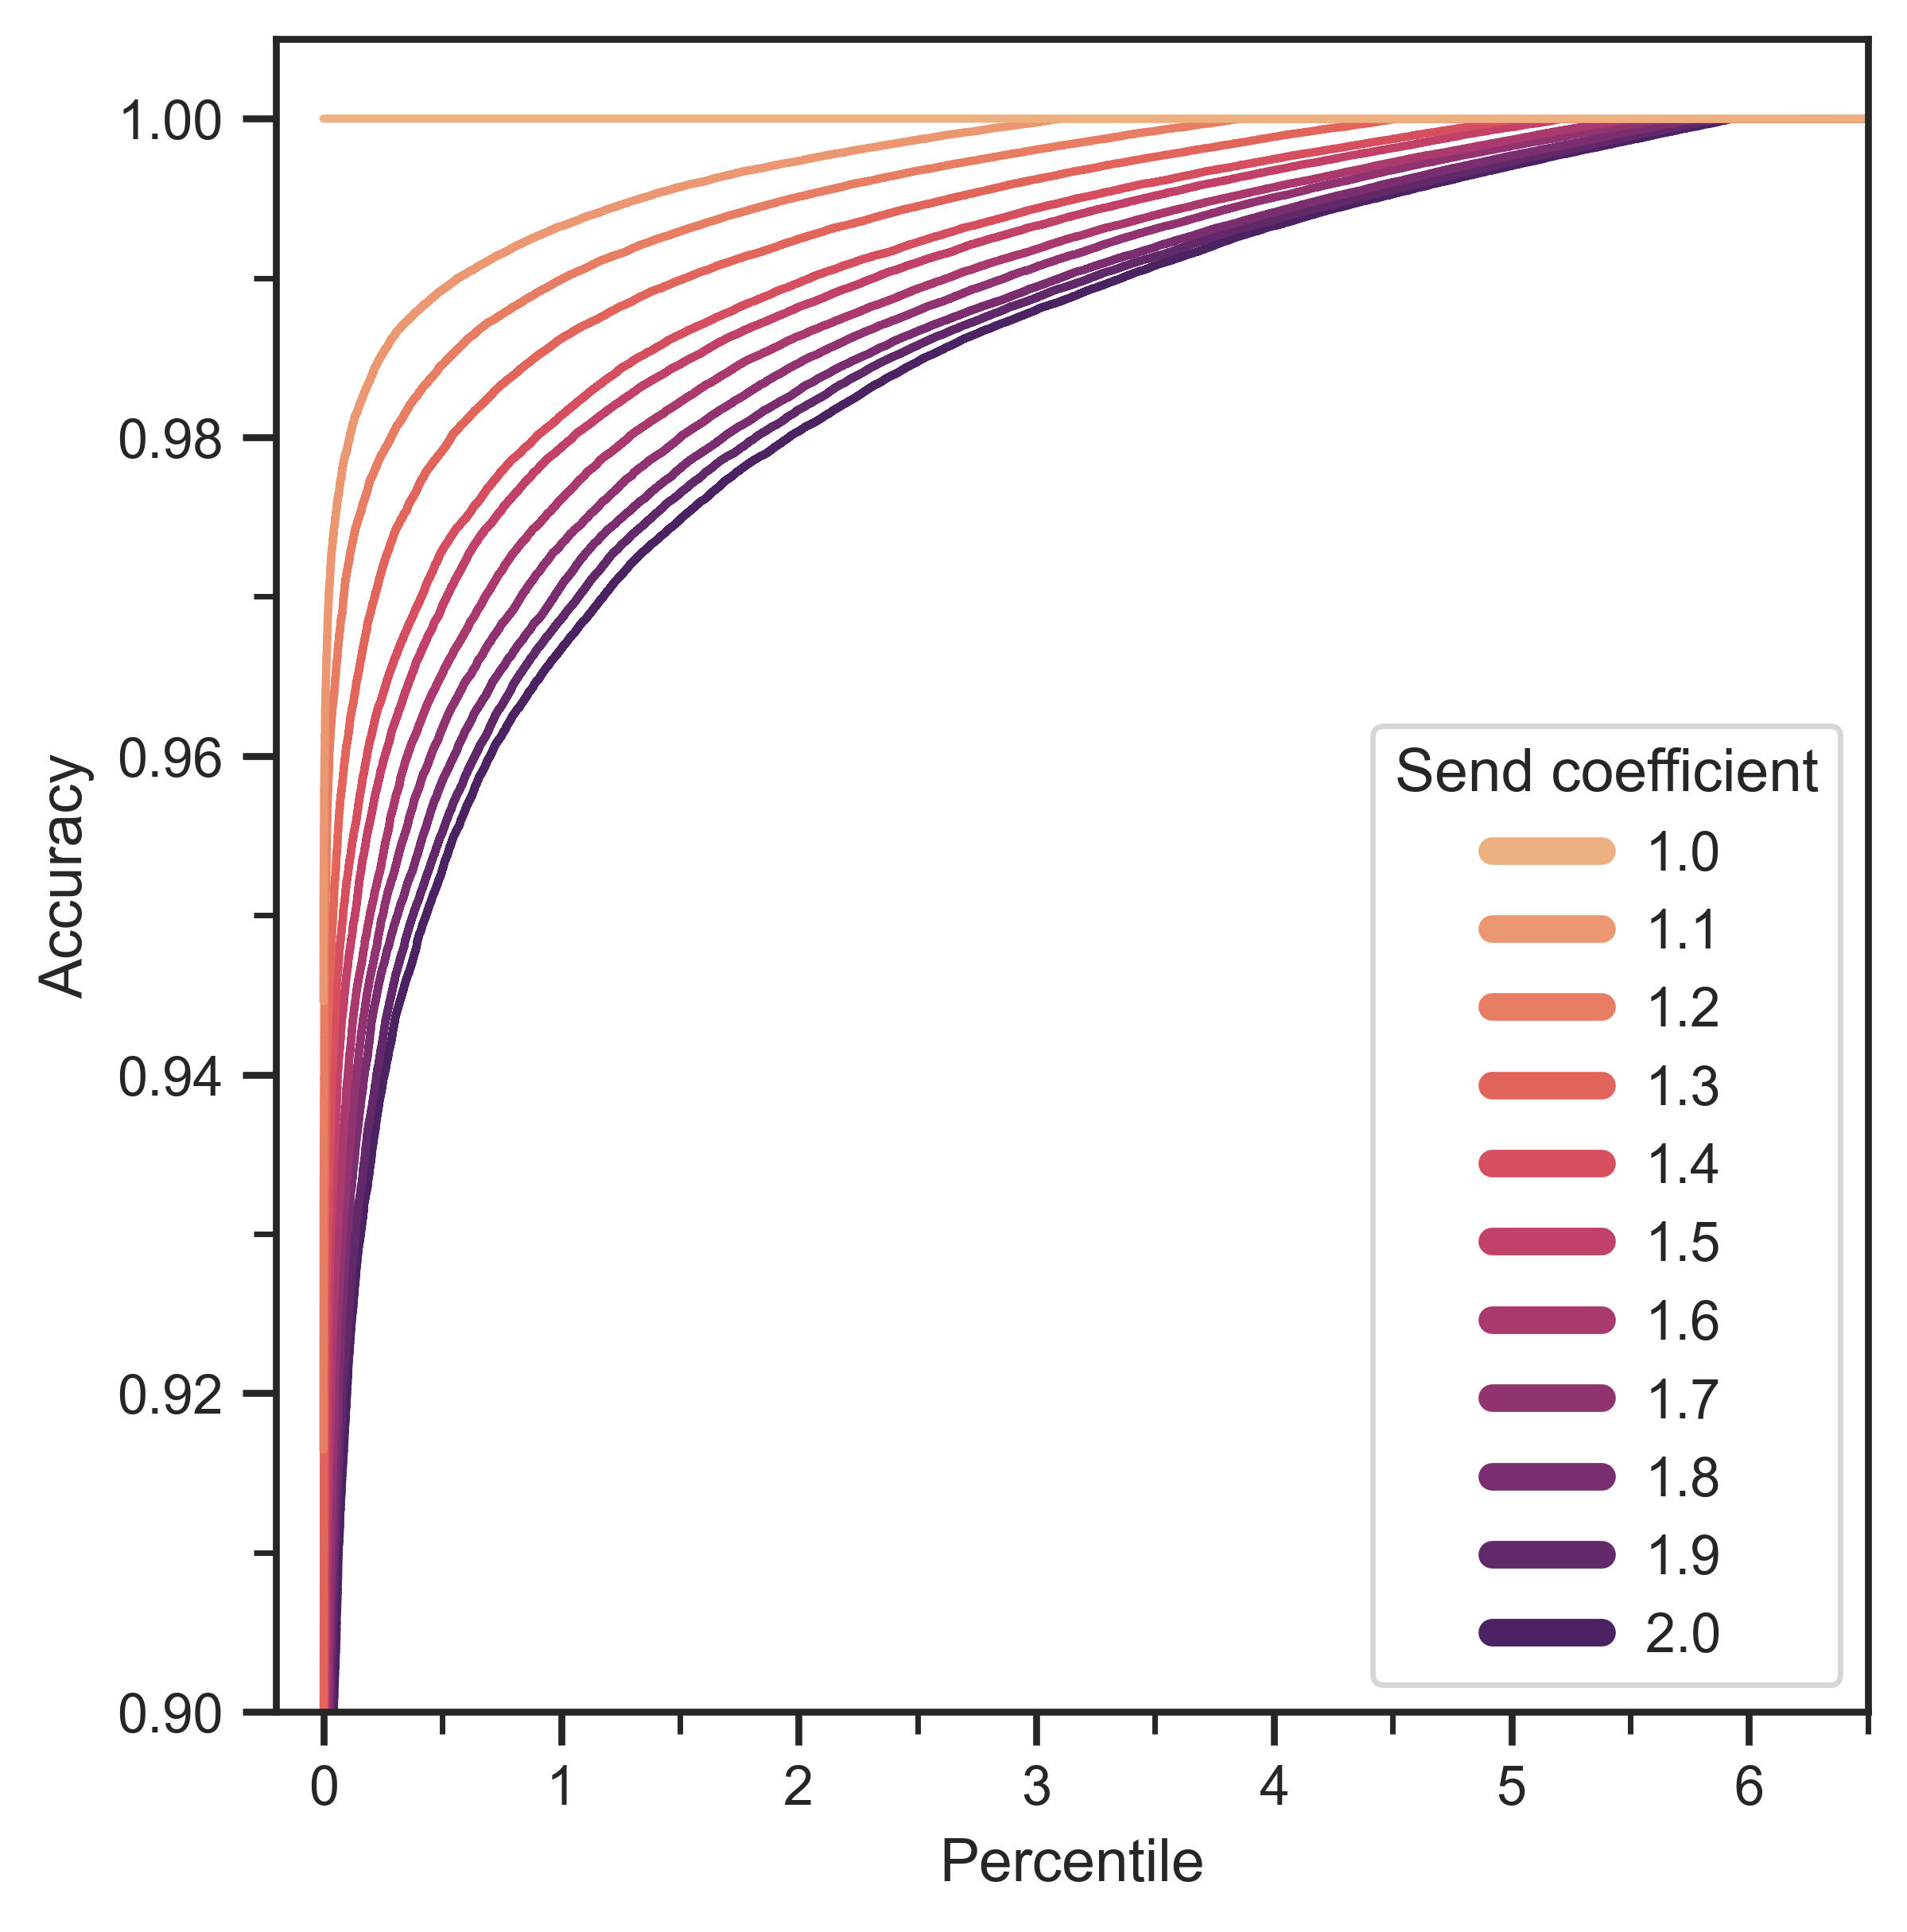
\includegraphics[width=\textwidth]{accuracy-percentiles}
  \caption[Cumulative accuracy distributions]{Cumulative accuracy distributions.}
  \label{fig:accuracy-percentiles}
\end{figure}

\begin{sidewaystable}[htbp]
\centering
\begin{tabular}{
  S
  S[table-auto-round, table-format = 1.3]
  S[table-auto-round, table-format = 1.3]
  S[table-auto-round, table-format = 1.3]
  S[table-auto-round, table-format = 1.3]
  S[table-auto-round, table-format = 1.3]
  S[table-auto-round, table-format = 1.3]
  S[table-auto-round, table-format = 1.3]
  S[table-auto-round, table-format = 1.3]
  S[table-auto-round, table-format = 1.3]
  S[table-auto-round, table-format = 1.3]
}
  \toprule
  {Send coefficient} & {$P_{0}$} & {$P_{0.01}$} & {$P_{0.1}$} & {$P_{1}$} & {$P_{2}$} & {$P_{3}$} & {$P_{4}$} & {$P_{5}$} & {$P_{6}$} & {$P_{21}$} \\
  \midrule
  0.8 & 0.724 & 0.802 & 0.844 & 0.871 & 0.889 & 0.903 & 0.914 & 0.924 & 0.933 & 1.0 \\
  0.9 & 0.903 & 0.926 & 0.937 & 0.968 & 0.986 & 0.993 & 0.997 & 0.999 & 1.0 & 1.0 \\
  1.0 & 1.0 & 1.0 & 1.0 & 1.0 & 1.0 & 1.0 & 1.0 & 1.0 & 1.0 & 1.0 \\
  1.1 & 0.945 & 0.965 & 0.979 & 0.993 & 0.997 & 1.0 & 1.0 & 1.0 & 1.0 & 1.0 \\
  1.2 & 0.916 & 0.952 & 0.972 & 0.99 & 0.995 & 0.998 & 1.0 & 1.0 & 1.0 & 1.0 \\
  1.3 & 0.883 & 0.937 & 0.961 & 0.986 & 0.992 & 0.996 & 0.999 & 1.0 & 1.0 & 1.0 \\
  1.4 & 0.882 & 0.922 & 0.952 & 0.981 & 0.99 & 0.994 & 0.997 & 1.0 & 1.0 & 1.0 \\
  1.5 & 0.86 & 0.911 & 0.947 & 0.979 & 0.988 & 0.993 & 0.997 & 0.999 & 1.0 & 1.0 \\
  1.6 & 0.855 & 0.9 & 0.94 & 0.976 & 0.986 & 0.992 & 0.996 & 0.999 & 1.0 & 1.0 \\
  1.7 & 0.848 & 0.891 & 0.934 & 0.973 & 0.985 & 0.991 & 0.995 & 0.998 & 1.0 & 1.0 \\
  1.8 & 0.84 & 0.884 & 0.93 & 0.971 & 0.983 & 0.989 & 0.994 & 0.998 & 1.0 & 1.0 \\
  1.9 & 0.826 & 0.879 & 0.924 & 0.969 & 0.982 & 0.989 & 0.994 & 0.997 & 1.0 & 1.0 \\
  2.0 & 0.817 & 0.871 & 0.92 & 0.967 & 0.98 & 0.988 & 0.993 & 0.997 & 1.0 & 1.0 \\
  \bottomrule
\end{tabular}
\caption[Accuracy percentiles]{Accuracy percentiles. The idle timeout (see \cref{tab:default-parameters}) was suspected to be insufficient for the executions associated with a send coefficient $\pSendCoefficient < 1$ to complete, but it is expected that $\pSendCoefficient \leq 1$ permit perfect accuracy.}
\label{tab:accuracy-percentiles}
\end{sidewaystable}

\Cref{fig:accuracy-percentiles} and \cref{tab:accuracy-percentiles} effectively describe the cumulative accuracy distributions of a population consisting of many disconnected contact networks. While that view can determine the accuracy \class{RiskPropagation} provides to a given percentile of the population, it does not quantify the extent to which a given send coefficient achieves perfect accuracy within each contact network. 

Let $\pSendCoefficient_i^*$ be the maximum send coefficient for \indexed{i}{individual of a repetition} that provides maximal accuracy,
\begin{equation*}
  \pSendCoefficient_i^* = \max \left(\underset{\pSendCoefficient}{\argmax} \, f_i(\pSendCoefficient)\right).
\end{equation*}
\Cref{fig:send-coefficient-optimality} and \cref{tab:send-coefficient-optimality} describe the proportion of individuals of each repetition that had a nonzero difference between their exposure score and symptom score, for which a given send coefficient was optimal. In other words, \cref{fig:send-coefficient-optimality} and \cref{tab:send-coefficient-optimality} describe the empirical upper bound distribution of network-wide accuracy for each send coefficient.

\begin{sidewaysfigure}[htbp]
  \centering
  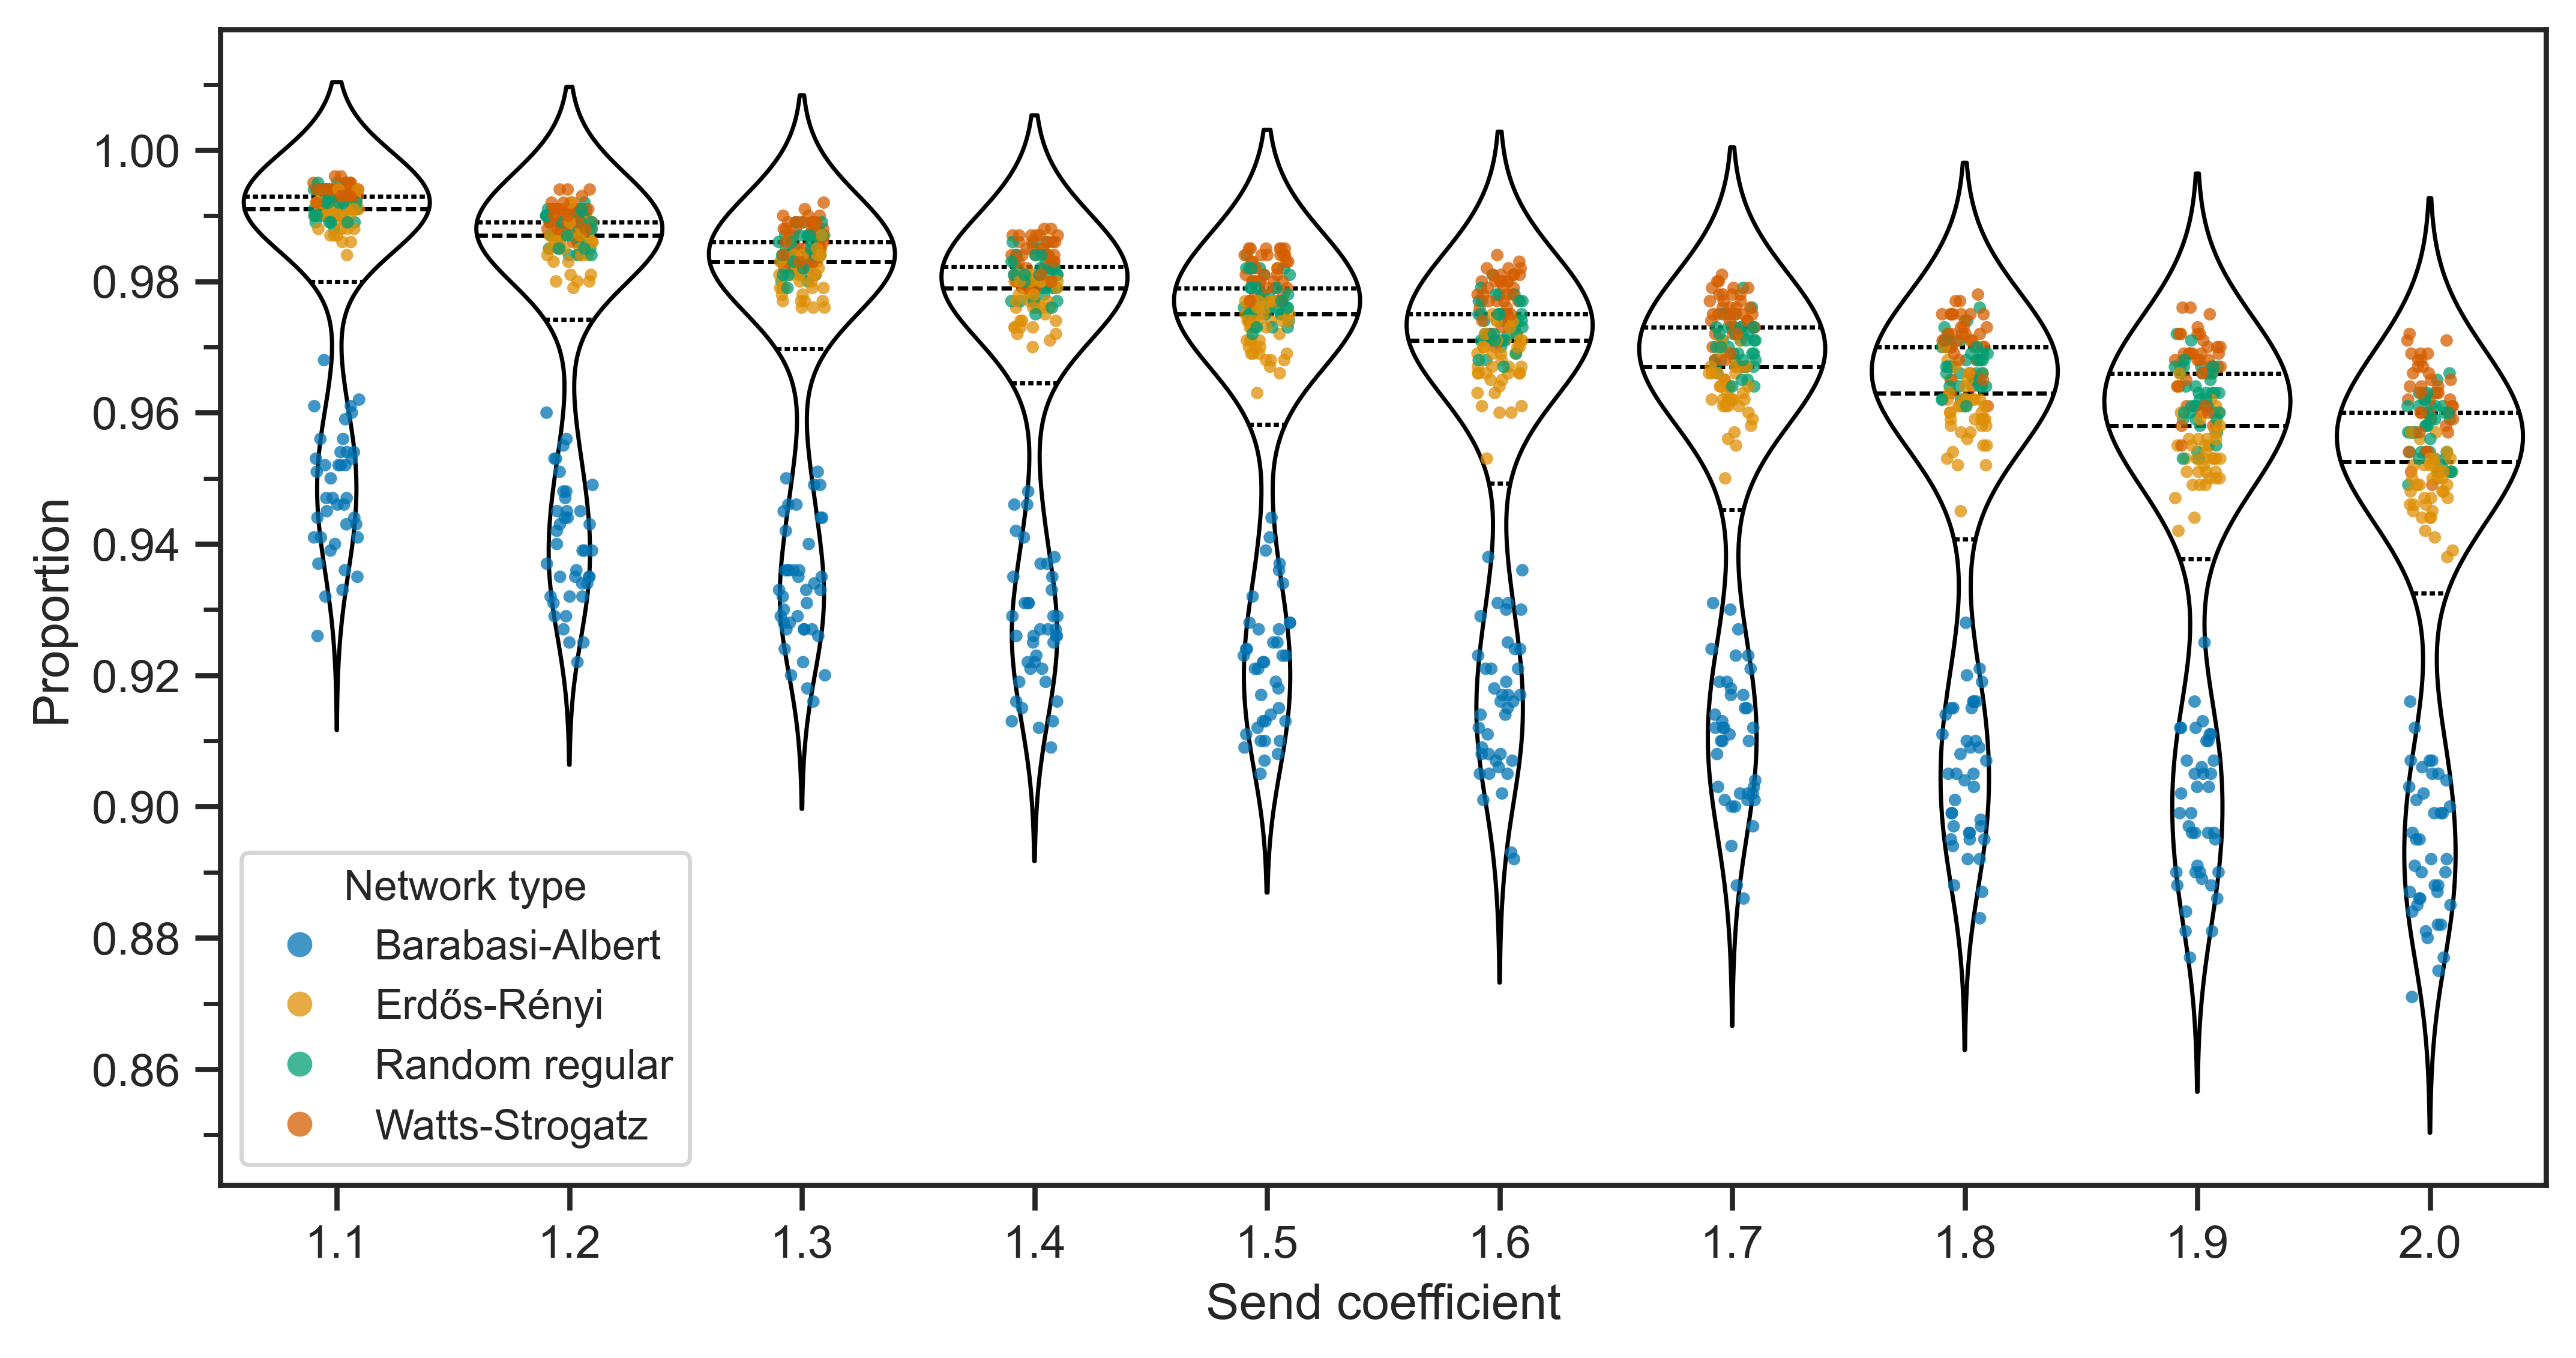
\includegraphics[width=\textwidth]{accuracy-proportions}
  \caption[Send coefficient optimality distributions]{Send coefficient optimality distributions. The dashed line inside each violin marks the median. The upper and lower dotted lines inside each violin mark the upper and lower quartiles, respectively.}
  \label{fig:send-coefficient-optimality}
\end{sidewaysfigure}

\begin{table}[htbp]
\centering
\begin{tabular}{
  S
  S[table-auto-round, table-format = 1.3]
  S[table-auto-round, table-format = 1.3]
  S[table-auto-round, table-format = 1.3]
  S[table-auto-round, table-format = 1.3]
  S[table-auto-round, table-format = 1.3]
  S[table-auto-round, table-format = 1.3]
  S[table-auto-round, table-format = 1.3]
}
  \toprule
  {Send coefficient} & {$P_{0}$} & {$P_{10}$} & {$P_{25}$} & {$P_{50}$} & {$P_{75}$} & {$P_{90}$} & {$P_{100}$} \\
  \midrule
  1.0 & 1.0 & 1.0 & 1.0 & 1.0 & 1.0 & 1.0 & 1.0 \\ 
  1.1 & 0.926 & 0.946 & 0.976 & 0.991 & 0.993 & 0.994 & 0.996 \\ 
  1.2 & 0.922 & 0.936 & 0.97 & 0.987 & 0.989 & 0.991 & 0.994 \\ 
  1.3 & 0.916 & 0.931 & 0.964 & 0.983 & 0.986 & 0.988 & 0.992 \\ 
  1.4 & 0.909 & 0.926 & 0.959 & 0.979 & 0.982 & 0.986 & 0.988 \\ 
  1.5 & 0.905 & 0.919 & 0.954 & 0.975 & 0.979 & 0.983 & 0.985 \\ 
  1.6 & 0.892 & 0.913 & 0.946 & 0.971 & 0.975 & 0.98 & 0.984 \\ 
  1.7 & 0.886 & 0.909 & 0.941 & 0.967 & 0.973 & 0.976 & 0.981 \\ 
  1.8 & 0.883 & 0.9 & 0.937 & 0.963 & 0.97 & 0.973 & 0.978 \\ 
  1.9 & 0.877 & 0.896 & 0.934 & 0.958 & 0.966 & 0.969 & 0.976 \\ 
  2.0 & 0.871 & 0.889 & 0.927 & 0.952 & 0.96 & 0.964 & 0.972 \\ 
  \bottomrule
\end{tabular}
\caption[Send coefficient optimality percentiles]{Send coefficient optimality percentiles.}
\label{tab:send-coefficient-optimality}
\end{table}

With respect to efficiency, \cref{fig:message-passing-efficiency} and \cref{tab:message-passing-efficiency} indicate that even modest increases above $\pSendCoefficient = 1$ can reduce the total number of messages received by \qtyrange{10}{20}{\percent} in a contact network. Larger increases above $\pSendCoefficient = 1$ can reduce the total number of messages received by up to \qty{30}{\percent}; however, accuracy should also be considered. \Cref{fig:message-reachability} indicates that message reachability is distributed consistently across network types. Though the proportion of individuals with a message reachability of 0 is inversely correlated with the send coefficient, the remainder of the cumulative distribution is nearly identical across send coefficients. \Cref{tab:message-reachability} describes several percentiles of the message reachability cumulative distribution, aggregating across send coefficients.

\begin{figure}[htbp]
  \centering
  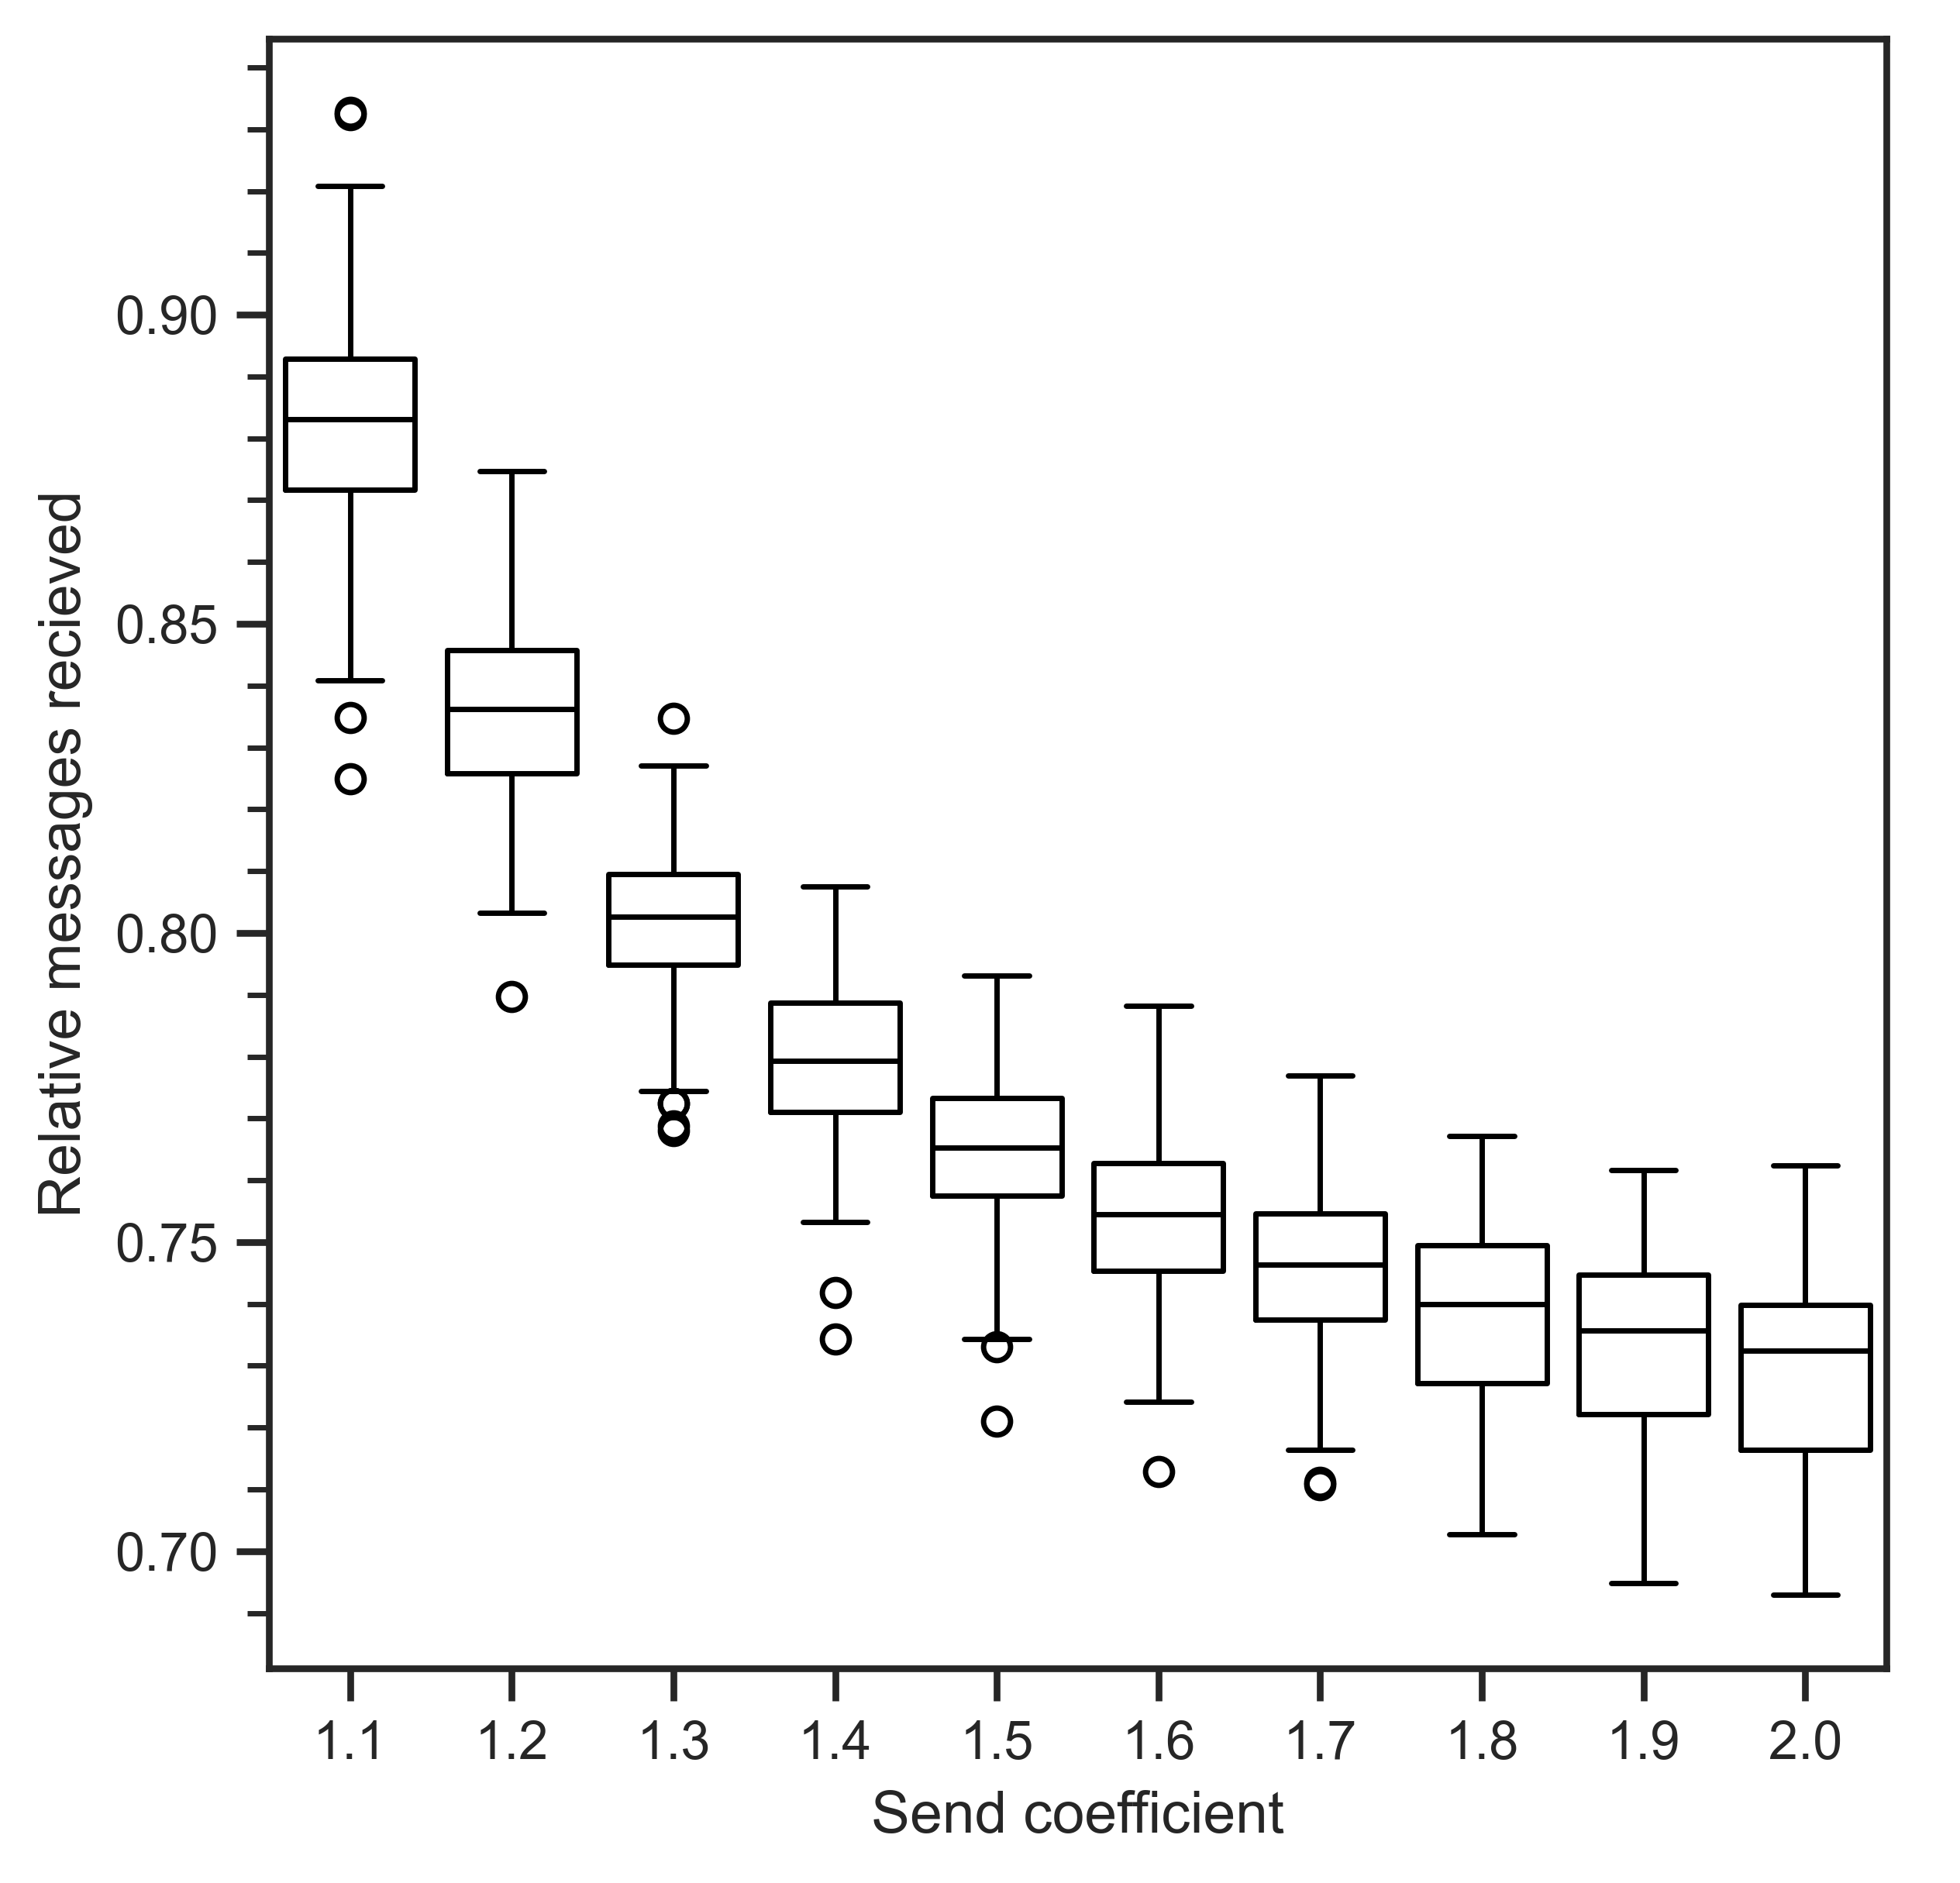
\includegraphics[width=\textwidth]{relative-receives}
  \caption[Message-passing efficiency]{Message-passing efficiency. The send coefficient $\pSendCoefficient = 1$ was used as a baseline for message-passing efficiency since it was found to be the maximum send coefficient that achieves perfect accuracy.}
  \label{fig:message-passing-efficiency}
\end{figure}

\begin{table}[htbp]
\centering
\begin{tabular}{
  S
  S[table-auto-round, table-format = 1.3]
  S[table-auto-round, table-format = 1.3]
  S[table-auto-round, table-format = 1.3]
  S[table-auto-round, table-format = 1.3]
  S[table-auto-round, table-format = 1.3]
  S[table-auto-round, table-format = 1.3]
  S[table-auto-round, table-format = 1.3]
}
  \toprule
  {Send coefficient} & {$P_{0}$} & {$P_{10}$} & {$P_{25}$} & {$P_{50}$} & {$P_{75}$} & {$P_{90}$} & {$P_{100}$} \\
  \midrule
  1.0 & 1.0 & 1.0 & 1.0 & 1.0 & 1.0 & 1.0 & 1.0 \\
  1.1 & 0.825 & 0.856 & 0.872 & 0.883 & 0.893 & 0.902 & 0.933 \\
  1.2 & 0.79 & 0.815 & 0.826 & 0.836 & 0.846 & 0.851 & 0.875 \\
  1.3 & 0.768 & 0.784 & 0.795 & 0.803 & 0.81 & 0.814 & 0.835 \\
  1.4 & 0.734 & 0.761 & 0.771 & 0.779 & 0.789 & 0.797 & 0.808 \\
  1.5 & 0.721 & 0.748 & 0.757 & 0.765 & 0.773 & 0.781 & 0.793 \\
  1.6 & 0.713 & 0.735 & 0.745 & 0.755 & 0.763 & 0.771 & 0.788 \\
  1.7 & 0.711 & 0.728 & 0.737 & 0.746 & 0.755 & 0.763 & 0.777 \\
  1.8 & 0.703 & 0.718 & 0.727 & 0.74 & 0.749 & 0.757 & 0.767 \\
  1.9 & 0.695 & 0.715 & 0.722 & 0.736 & 0.745 & 0.752 & 0.762 \\
  2.0 & 0.693 & 0.707 & 0.716 & 0.732 & 0.74 & 0.749 & 0.762 \\
  \bottomrule
\end{tabular}
\caption[Relative messages received percentiles]{Relative messages received percentiles.}
\label{tab:message-passing-efficiency}
\end{table}


\begin{figure}[htbp]
  \centering
  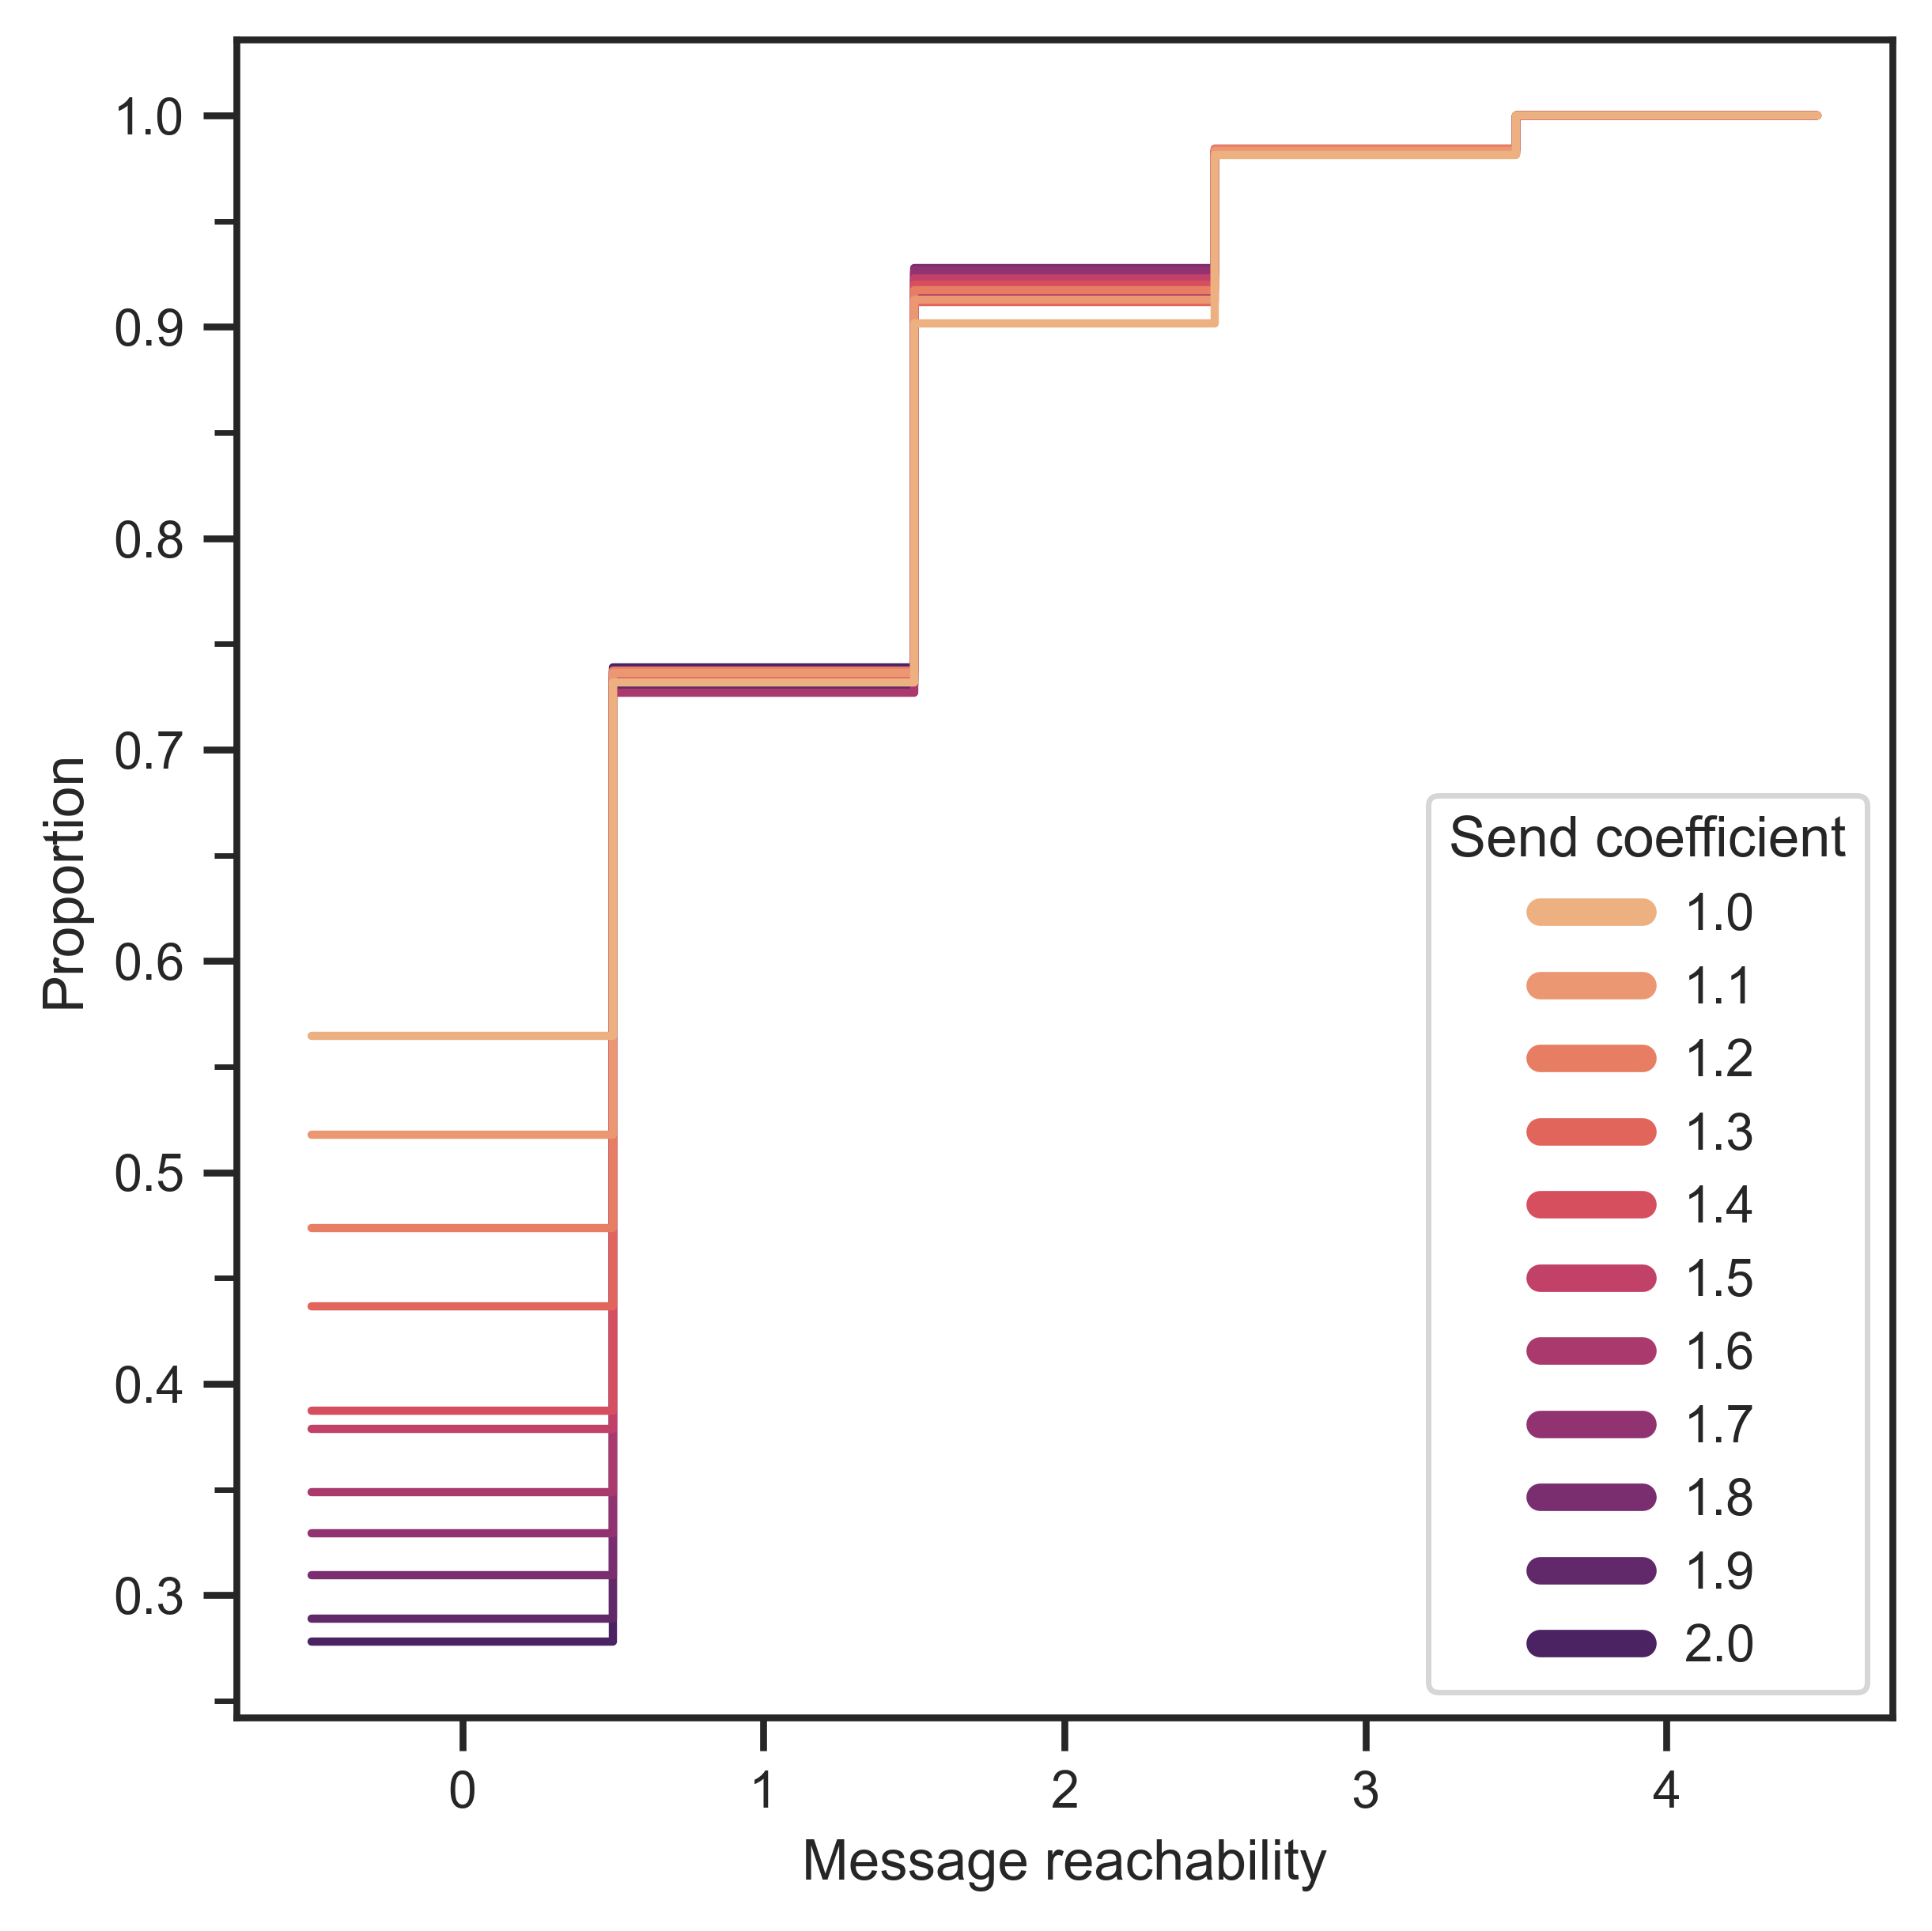
\includegraphics[width=\textwidth]{message-reachability}
  \caption[Message reachability cumulative distributions]{Message reachability cumulative distributions.}
  \label{fig:message-reachability}
\end{figure}

\begin{table}[htbp]
\centering
\begin{tabular}{SSSSSSSSS}
  \toprule
  {$P_{25}$} & {$P_{50}$} & {$P_{75}$} & {$P_{90}$} & {$P_{95}$} & {$P_{99}$} & {$P_{99.9}$} & {$P_{99.99}$} & {$P_{100}$} \\
  \midrule
  0 & 1 & 2 & 2 & 3 & 4 & 5 & 7 & 9 \\
  \bottomrule
\end{tabular}
\caption[Message reachability percentiles]{Message reachability percentiles.}
\label{tab:message-reachability}
\end{table}

A brief exploratory analysis is provided to conclude this section. \Cref{tab:network-degree-percentiles} and \cref{fig:network-degree-distributions} and  describe the degree distributions of the contact networks that were used for this experiment. While other degree distributions are centered around 20, the Barabasi-Albert distribution is characterized by a power law that arises from the mechanism of preferential attachment. \Cref{fig:correlation-matrix} is the correlation matrix of the dataset attributes.

\begin{figure}[htbp]
  \centering
  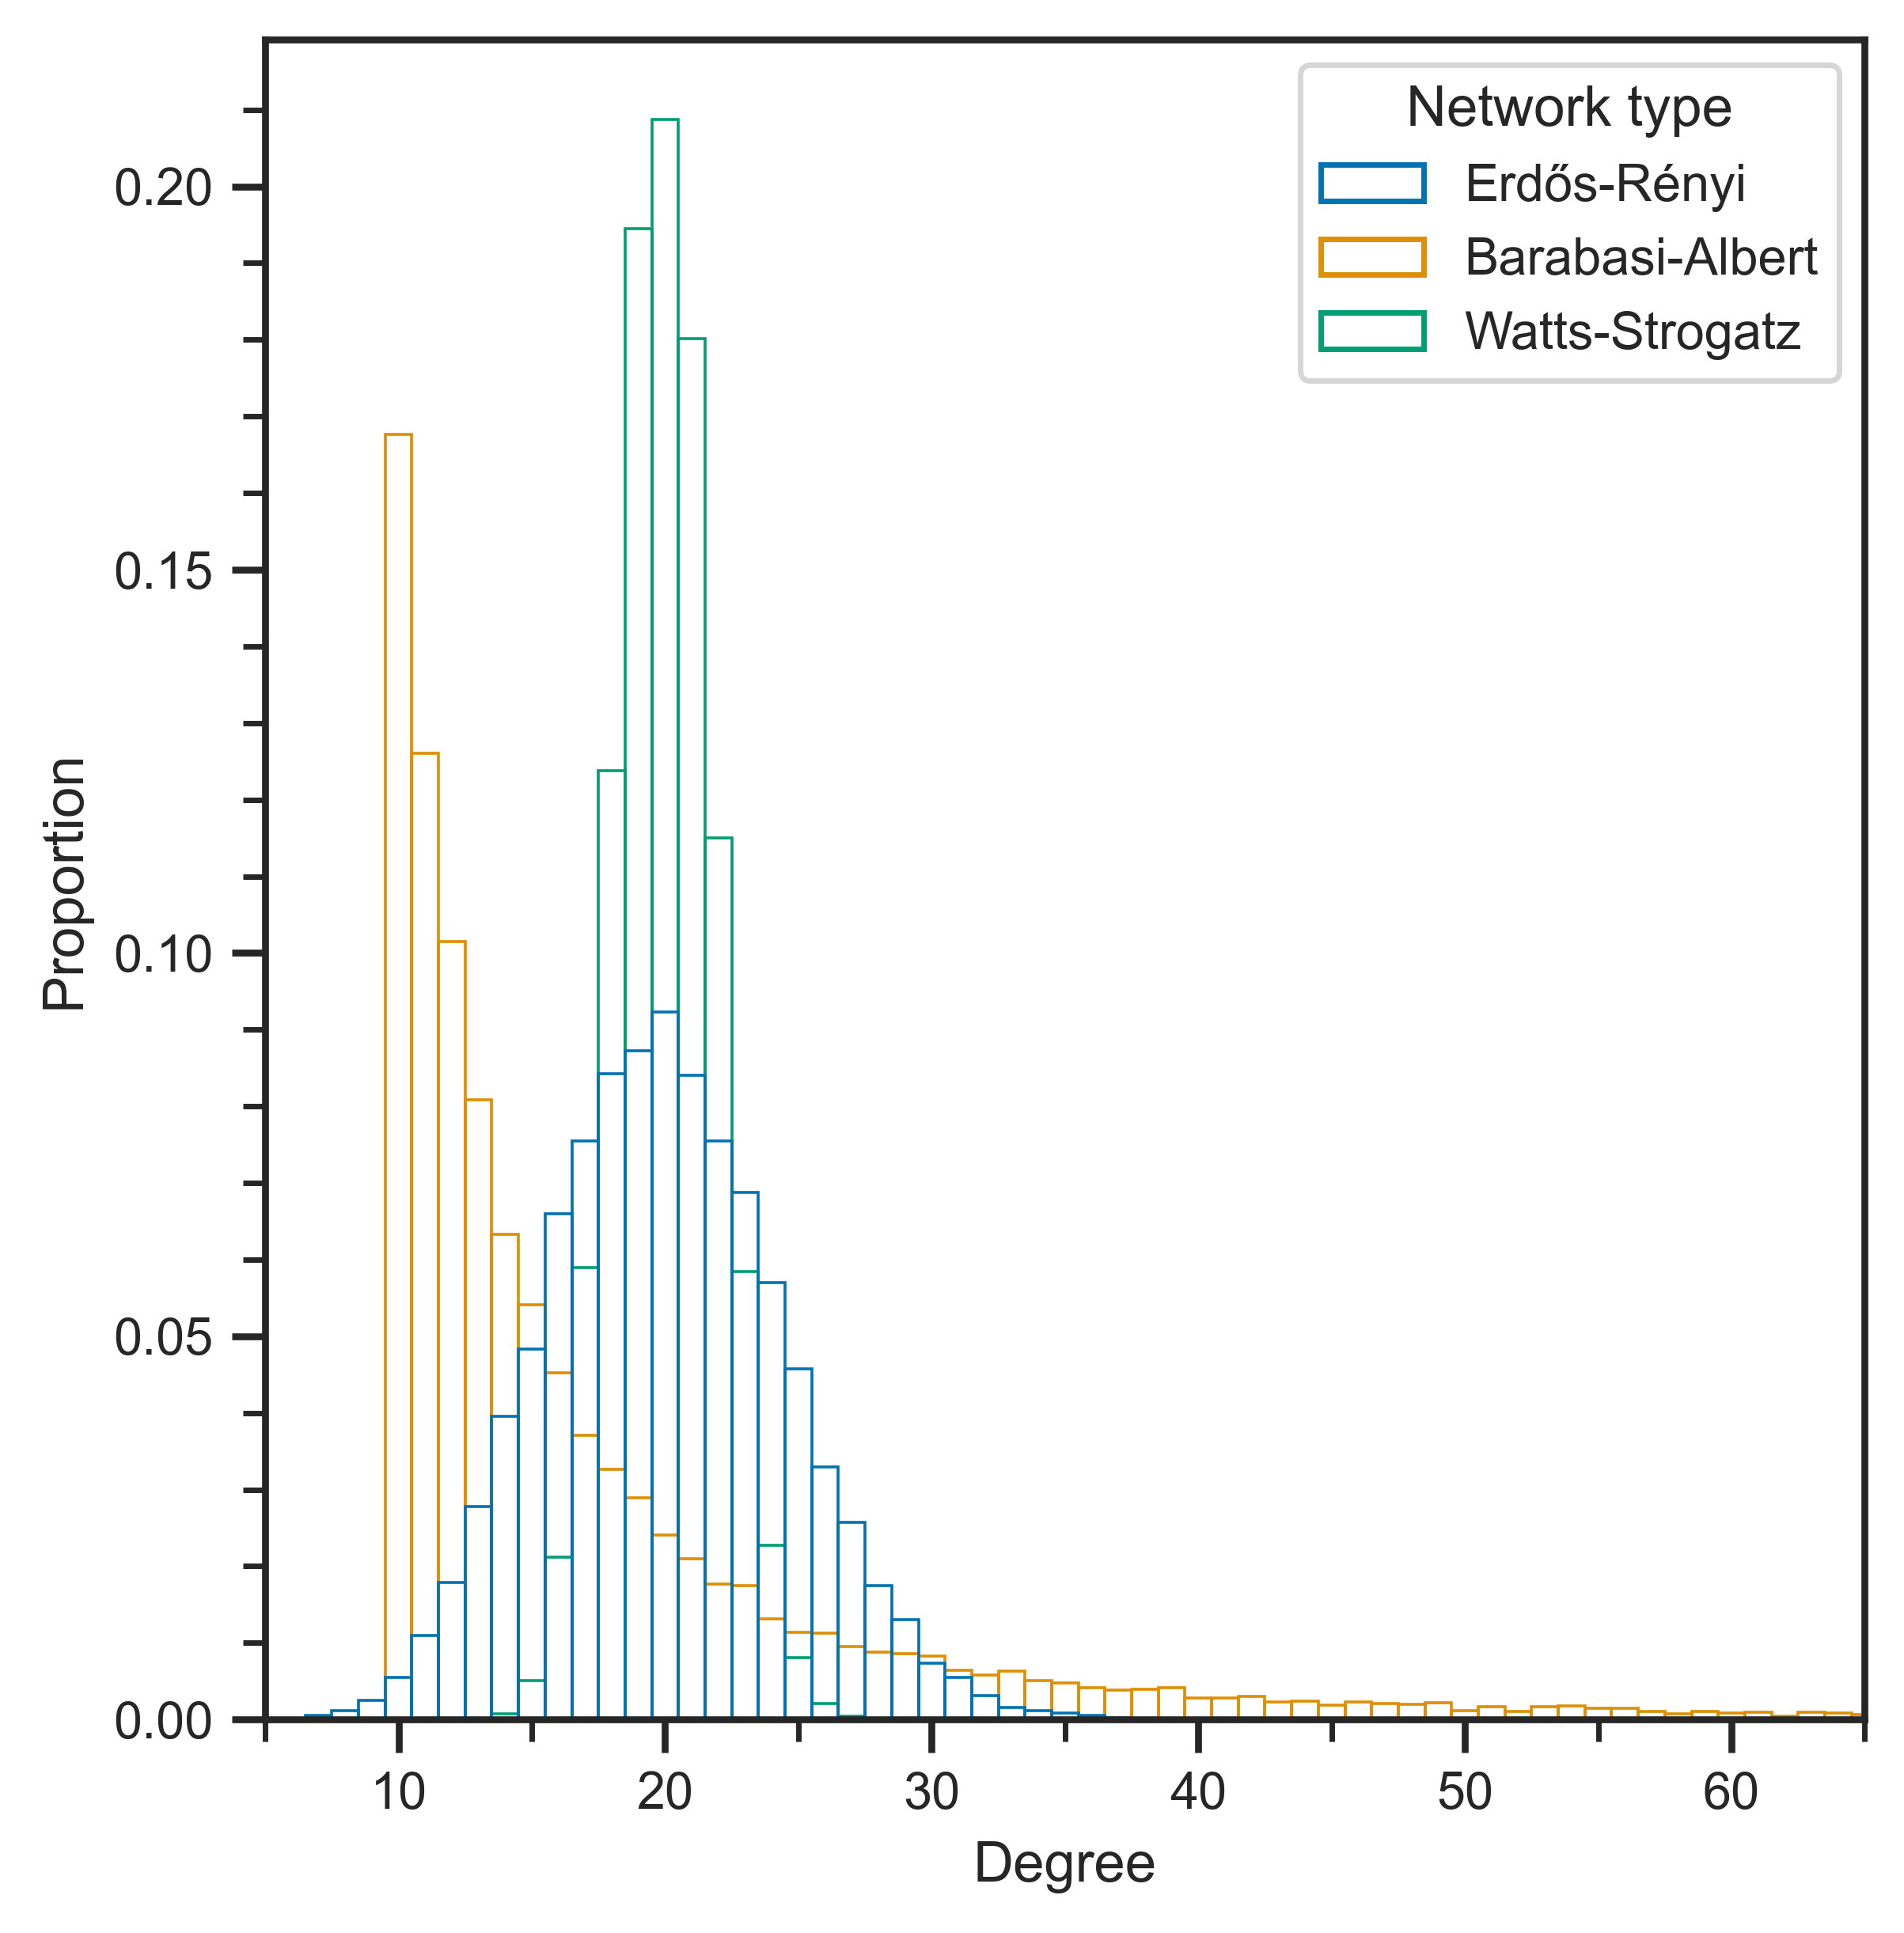
\includegraphics[width=\textwidth]{network-degree-distributions}
  \caption[Contact network degree distributions]{Contact network degree distributions. All \verticesName in random regular contact networks had a degree of 20, so the distribution was omitted to provide more visual space for the distributions of other contact networks.}
  \label{fig:network-degree-distributions}
\end{figure}

\begin{table}[htbp]
\centering
\begin{tabular}{lSSSSSSS}
  \toprule
  Network type & {$P_{0}$} & {$P_{10}$} & {$P_{25}$} & {$P_{50}$} & {$P_{75}$} & {$P_{90}$} & {$P_{100}$} \\
  \midrule
  Barabasi-Albert & 10 & 10 & 11 & 14 & 20 & 32 & 412 \\
  Erd\H{o}s-R\'{e}nyi & 5 & 14 & 17 & 20 & 23 & 26 & 38 \\
  Random regular & 20 & 20 & 20 & 20 & 20 & 20 & 20 \\
  Watts-Strogatz & 14 & 18 & 19 & 20 & 21 & 22 & 29 \\
  \bottomrule
\end{tabular}
\caption[Contact network degree percentiles]{Contact network degree percentiles.}
\label{tab:network-degree-percentiles}
\end{table}

\begin{figure}[htbp]
  \centering
  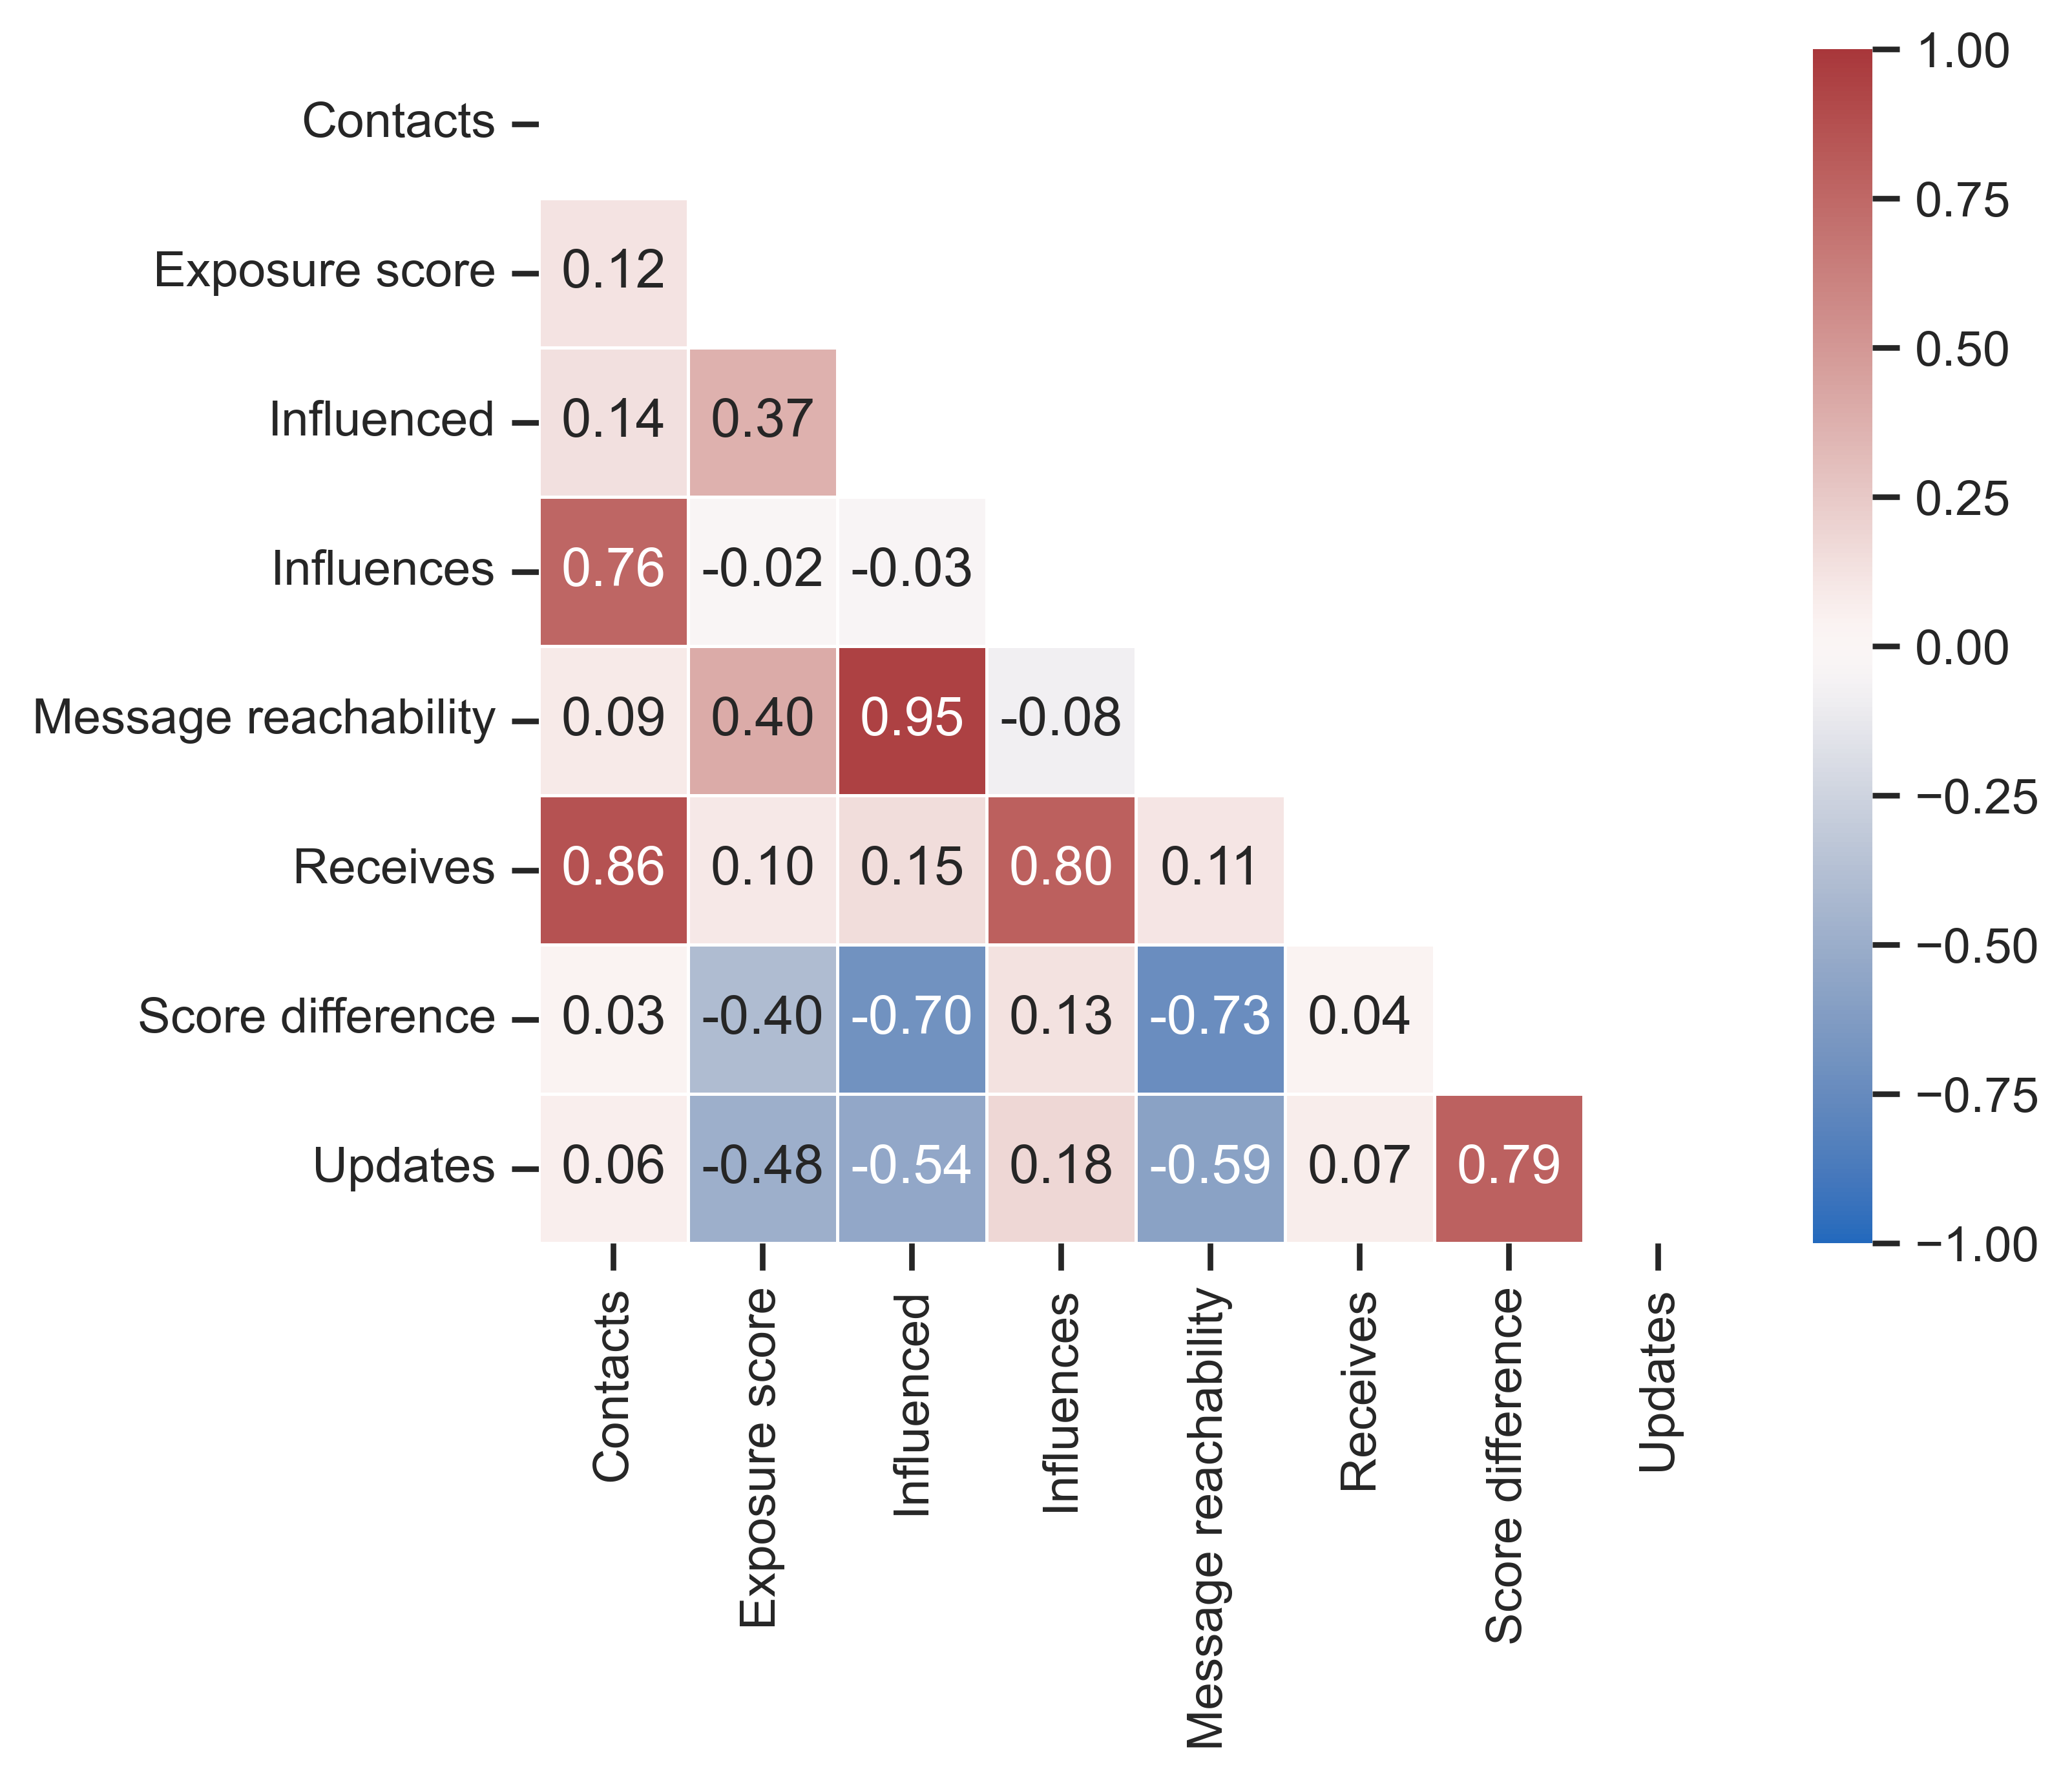
\includegraphics[width=\textwidth]{correlation}
  \caption[Correlation matrix of \labelcref{item:parameters} dataset attributes]{Correlation matrix of \labelcref{item:parameters} dataset attributes. Each cell is the Spearman rank partial correlation coefficient \citep{Spearman1904}, controlling for the effect of the send coefficient. All coefficients are significant ($p < 0.01$), adjusting for multiple comparisons via the Holm–Bonferroni method \citep{Holm1979}.}
  \label{fig:correlation-matrix}
\end{figure}

\subsection{\labelcref{item:distributions}}\label{sec:runtime-baseline-experiment}

A one-way analysis of variance (ANOVA) was considered for determining if the mean message-passing runtimes associated with different data distributions are statistically different. ANOVA assumes the observations are independently sampled, normally distributed, and homoscedastic within groups. The message-passing runtimes were indeed independently sampled. To test the latter two assumptions, the Shapiro-Wilk test \citep{Shapiro1965} and the Fligner-Killeen test \citep{Fligner1976} were applied, respectively. While the runtimes were found to be homoscedastic ($p > \num{0.01}$), they were not normally distributed ($p < \num{0.01}$). As such, the Kruskal-Wallis test was applied instead of a one-way ANOVA. The test indicated that there is insufficient evidence to reject the null hypothesis that the median message-passing runtimes are the same across data distributions. See \cref{tab:runtime-hypothesis-tests} for the test statistics and associated $p$-values. Note, this experiment assumes this statistical nonsignificance holds for other data distributions and network topologies.

\begin{sidewaystable}[htbp]
\centering
\begin{tabular}{lSSSSSS}
  \toprule
  & \multicolumn{2}{c}{Shapiro-Wilk test} & \multicolumn{2}{c}{Fligner-Killeen test} & \multicolumn{2}{c}{Kruskal-Wallis test} \\
  \cmidrule(lr){2-3} \cmidrule(lr){4-5} \cmidrule(lr){6-7}
  Network type & {Statistic} & {$p$-value} & {Statistic} & {$p$-value} & {Statistic} & {$p$-value} \\
  \midrule
  All & 0.672 & {$<\num{0.01}$} & 2.26 & 0.944 & 7.03 & 0.426 \\
  Barabasi-Albert & 0.646 & {$<\num{0.01}$} & 4.54 & 0.716 & 5.24 & 0.631 \\
  Erd\H{o}s-R\'{e}nyi & 0.472 & {$<\num{0.01}$} & 4.87 & 0.676 & 3.23 & 0.863 \\
  Random regular & 0.583 & {$<\num{0.01}$} & 3.90 & 0.791 & 3.02 & 0.883 \\
  Watts-Strogatz & 0.437 & {$<\num{0.01}$} & 2.47 & 0.929 & 5.97 & 0.543 \\
  \bottomrule
\end{tabular}
\caption[Hypothesis tests for message-passing runtime]{Hypothesis tests for message-passing runtime.}
\label{tab:runtime-hypothesis-tests}
\end{sidewaystable}

\subsection{\labelcref{item:topology}}\label{sec:runtime-experiment}

\Cref{fig:runtimes} indicates a linear relationship exists between the message-passing runtime and the size of the contact network. Given the runtime variance is heteroscedastic, quantile regression \citep{Koenker1978} was applied to determine the linear models that describe the $q = 0.05, 0.50, 0.95$ conditional quantiles of the message-passing runtime,
\begin{equation}\label{eq:runtime-model}
  f_q(x) = \beta_{0} + \beta_{1} x.
\end{equation}

\begin{sidewaysfigure}[htbp]
  \centering
  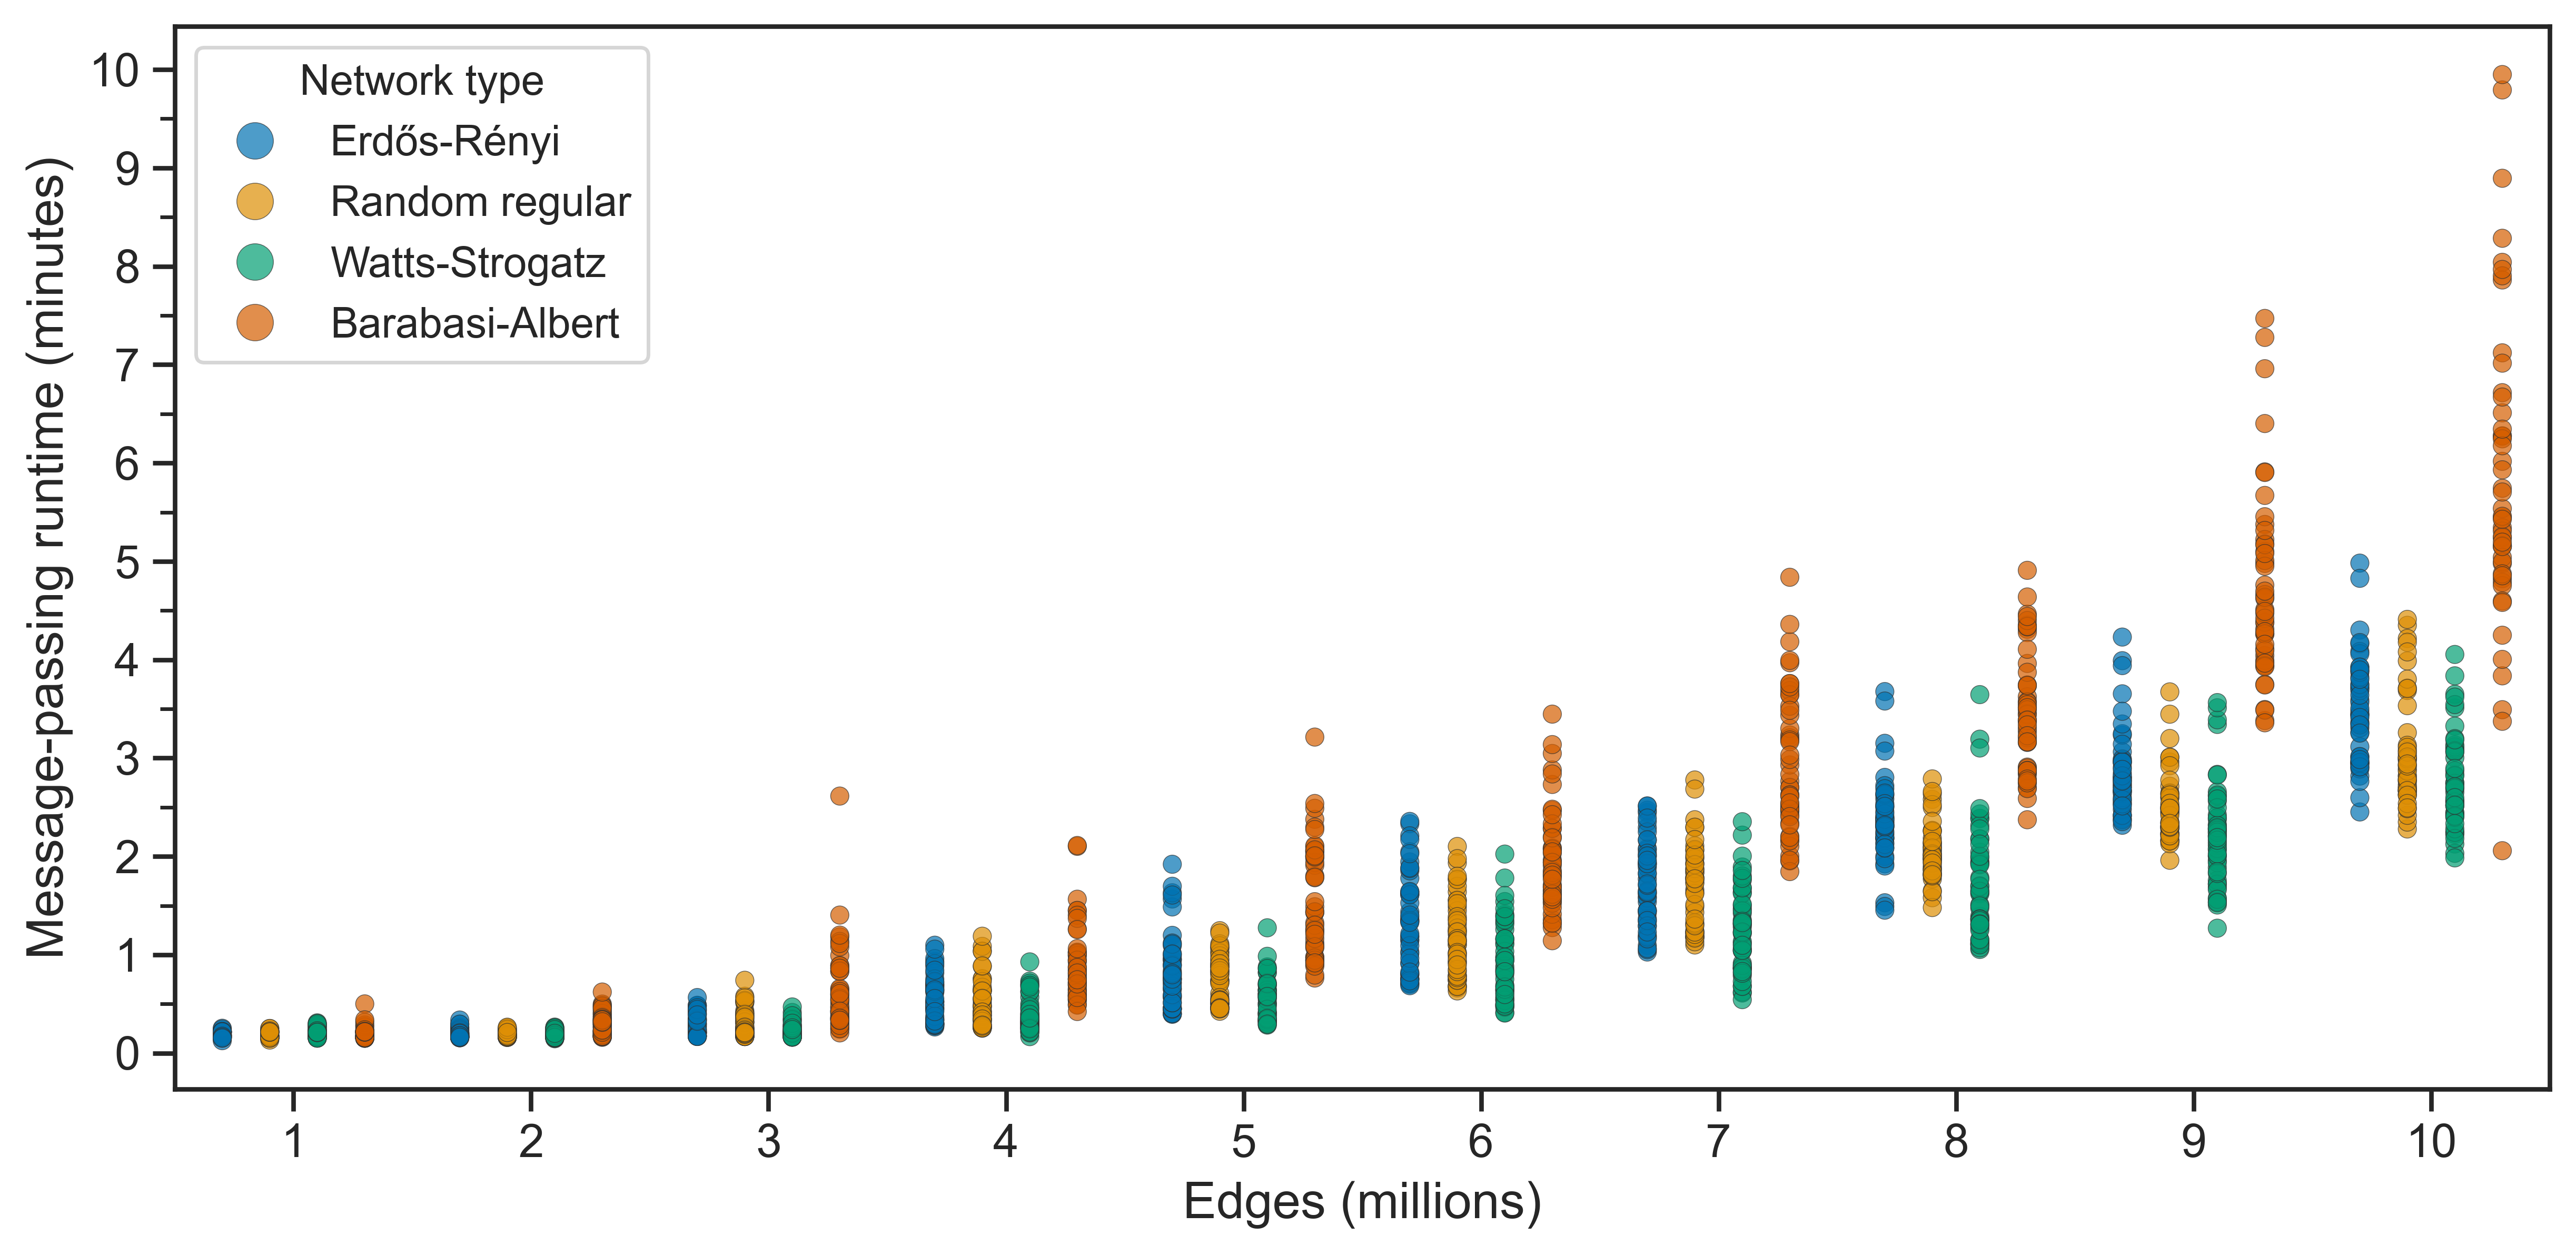
\includegraphics[width=\textwidth]{runtimes}
  \caption[Message-passing runtimes]{Message-passing runtimes.}
  \label{fig:runtimes}
\end{sidewaysfigure}

The pinball loss function \citep{Takeuchi2006} with $L_1$ regularization,
\begin{equation*}
  L(\mathbf{y}, \hat{\mathbf{y}}) = \rho(\mathbf{y}, \hat{\mathbf{y}}) + \lambda \|\hat{\boldsymbol{\beta}} \|_1,
\end{equation*}
was utilized for parameter estimation, where
\begin{equation*}
  \rho(\mathbf{y}, \hat{\mathbf{y}}) = \frac{1}{n} \sum_{i=1}^{n} \begin{cases}
    q(y_i - \hat{y}_i) & \text{if $y_i \geq \hat{y}_i$} \\
    (1 - q)(\hat{y}_i - y_i) & \text{otherwise}, \\
  \end{cases}
\end{equation*}
and $y_i, \hat{y}_i$ are the true and predicted message-passing runtimes associated with the network size $x_i$. Nested 5-fold cross validation \citep{Cawley2010} was applied for model selection (inner loop) and model assessment (outer loop) \cite[p. 222]{Hastie2009}. As part of model selection, grid search was applied over the set $\setBuilder{10^{-x}}{x \in \intInterval{1}{5}}$ to find the optimal regularization parameter $\lambda$. In addition to the mean pinball loss, the fraction of explained pinball deviance \citep{Koenker1999, Hastie2015} was calculated to provide a normalized measure for goodness of fit,
\begin{equation*}
  D^2(\mathbf{y}, \hat{\mathbf{y}}) = 1 - \frac{\rho(\mathbf{y}, \hat{\mathbf{y}})}{\rho(\mathbf{y}, \hat{\mathbf{y}}_0)},
\end{equation*}
where $\hat{\mathbf{y}}_0 = Q(\mathbf{y}, q) \cdot \mathbf{1}$ is the null model for the \indexed{q}{quantile}.

\Cref{tab:runtime-regression} specifies the optimal models and evaluation metrics. \Cref{fig:runtime-regression} overlays the observed message-passing runtimes with the predicted runtime quantiles.

\begin{table}[htbp]
\centering
  \begin{tabular}{
    S[table-format=1.3]
    S[table-format=-1.3]
    S[table-format=1.3e-2]
    S[table-format=1.3]
    S[table-format=-1.3]
    S[table-format=1.3]
    S[table-format=1.3]
    S[table-format=1.3]
  }
  \toprule
  &&&& \multicolumn{2}{c}{$\rho$} & \multicolumn{2}{c}{$D^2$} \\
  \cmidrule(lr){5-6} \cmidrule(lr){7-8}
  {$q$} & {$\beta_0$ (\unit{\second})} & {$\beta_1$ (edges / \unit{\second})} & {$\lambda$} & {Mean} & {SE} & {Mean} & {SE} \\
  \midrule
  0.05 & -34.1 & 1.25e-5 & 0.1 & -2.94 & 0.05 & 0.255 & 0.011 \\
  0.50 & -29.7 & 1.99e-5 & 0.1 & -15.6 & 0.4 & 0.520 & 0.009 \\
  0.95 & -21.7 & 3.48e-5 & 0.1 & -5.91 & 0.30 & 0.496 & 0.018 \\
  \bottomrule
  \end{tabular}
  \caption[Models of message-passing runtime]{Models of message-passing runtime. For \indexed{q}{quantile}, each row specifies the model parameters $\beta_0, \beta_1$ of \cref{eq:runtime-model} and the $L_1$ regularization parameter $\lambda$ that maximized the fraction of explained pinball deviance $D^2$ on the test set during model assessment. The mean and standard error (SE) of the pinball loss $\rho$ and $D^2$ are also provided from model assessment.
}
  \label{tab:runtime-regression}
\end{table}

\begin{figure}[htbp]
  \centering
  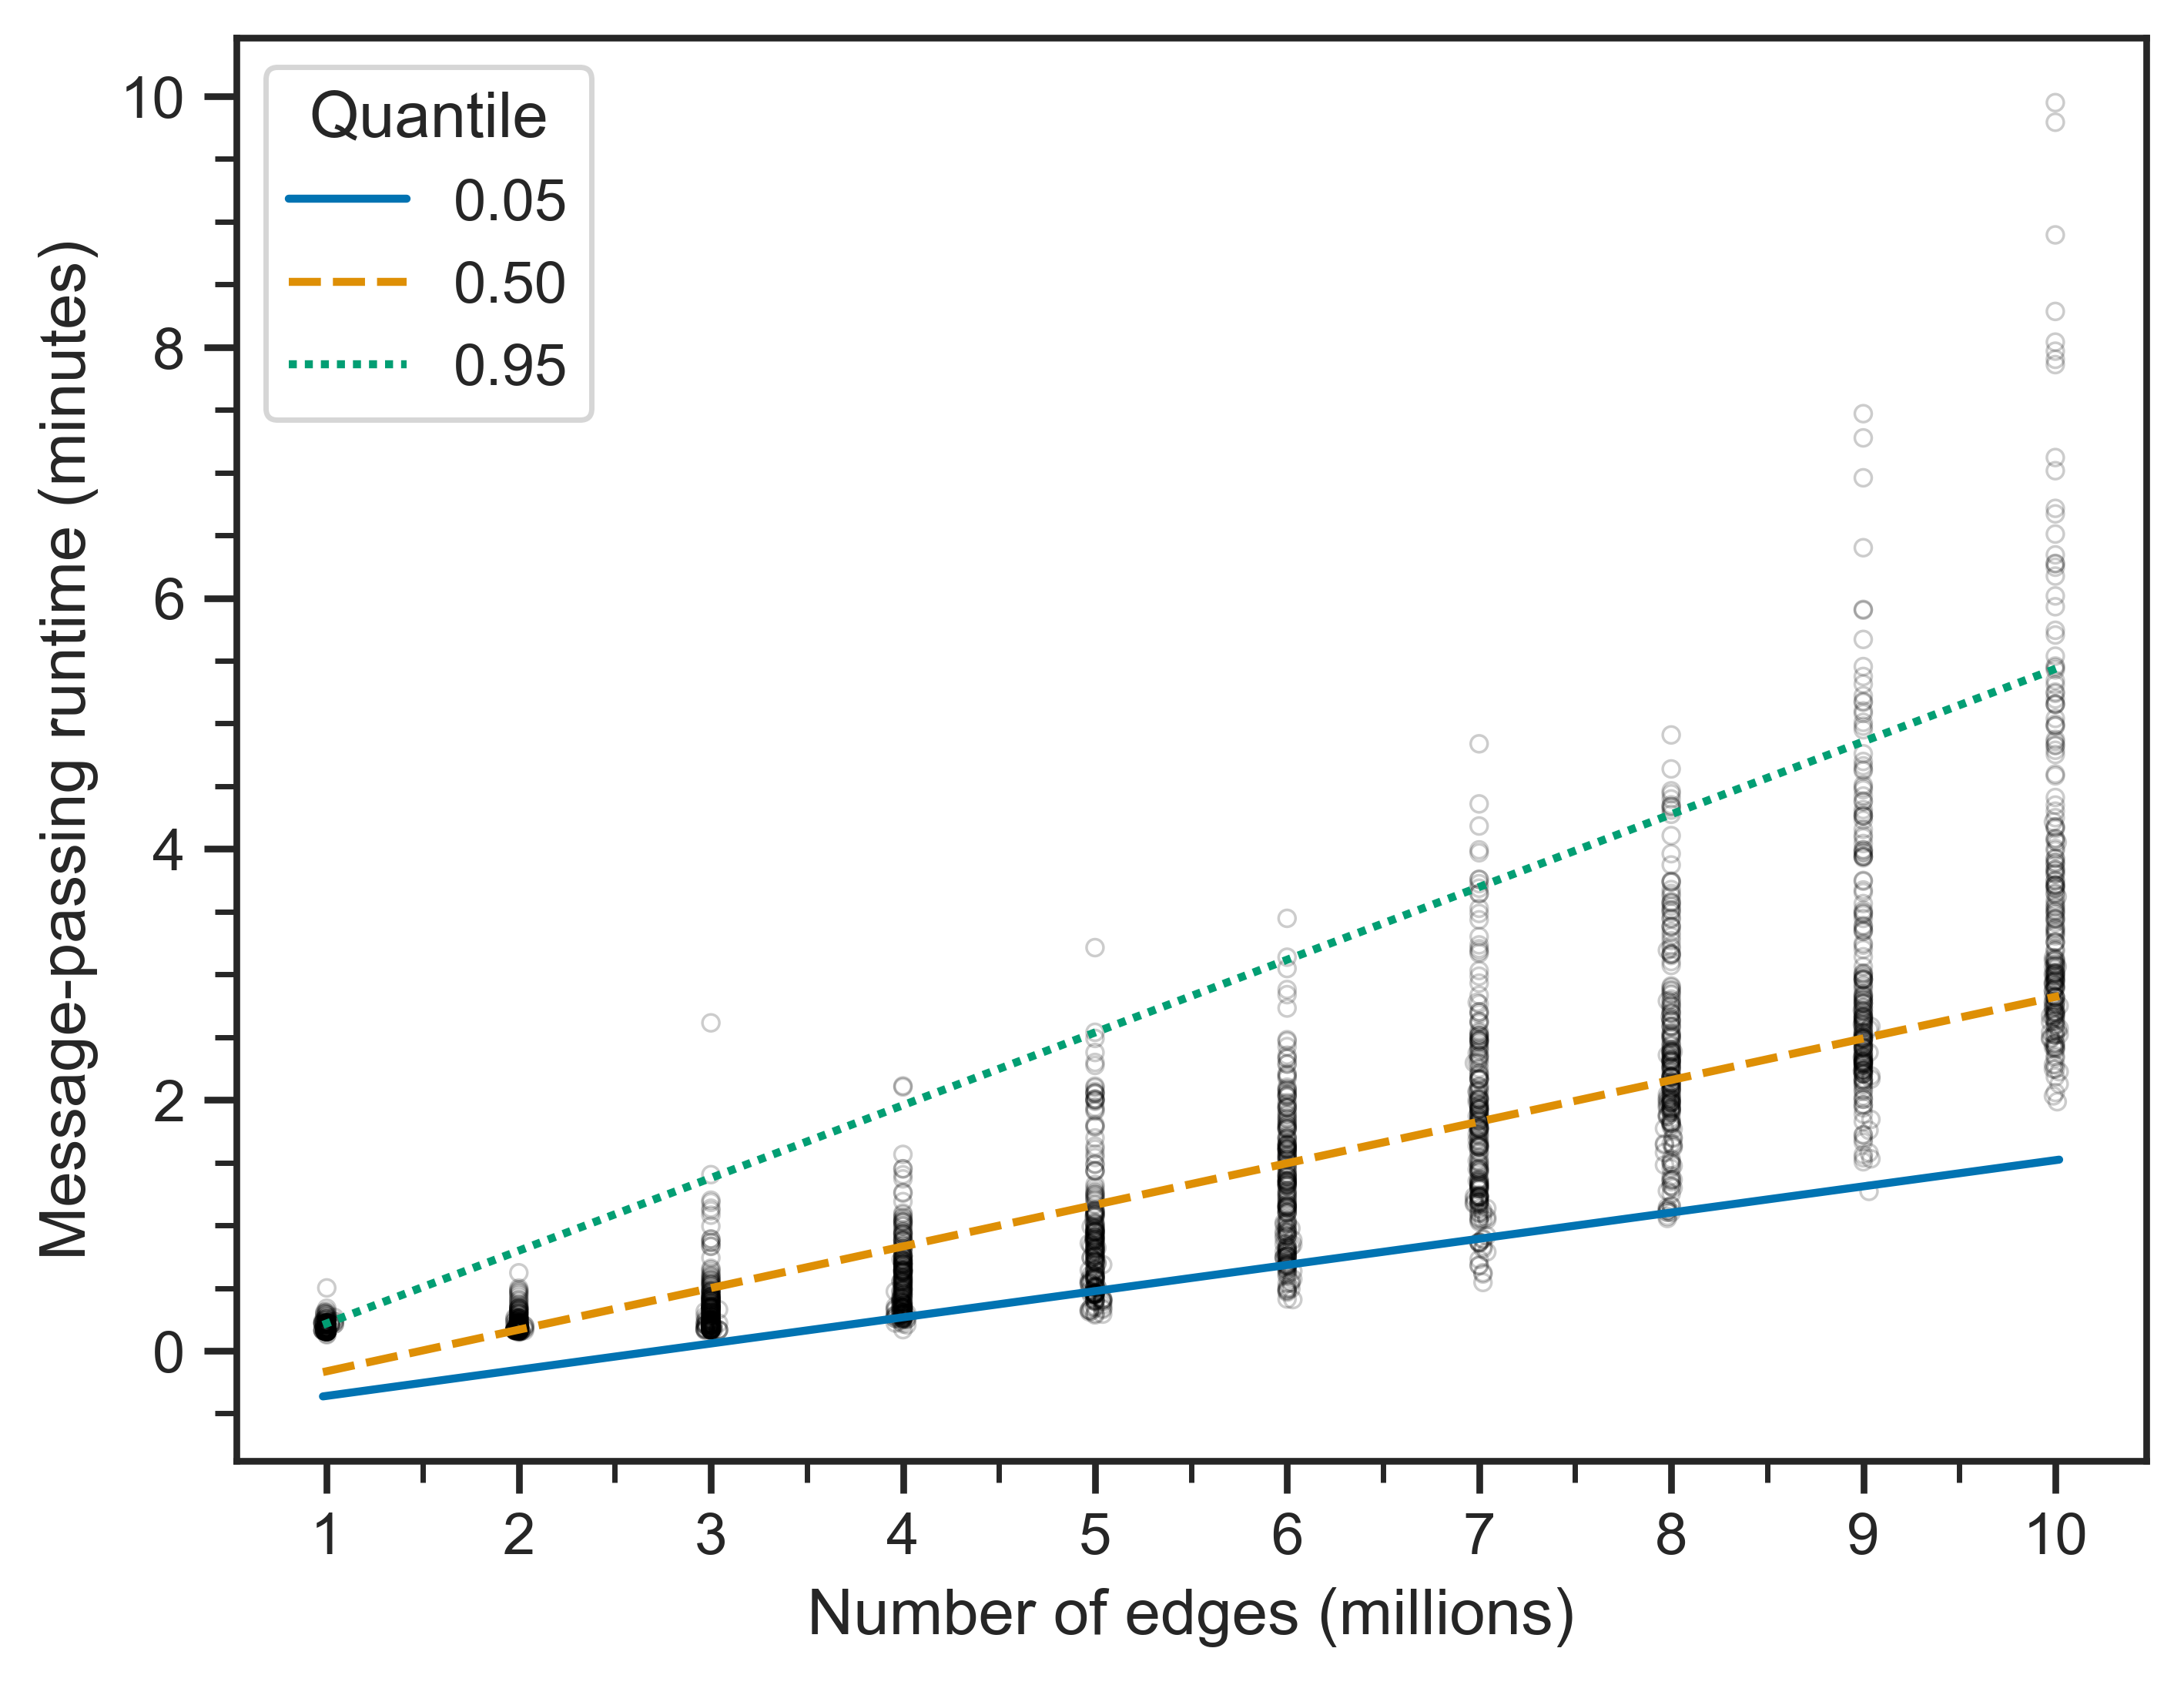
\includegraphics[width=\textwidth]{runtime-regression}
  \caption[Message-passing runtimes with regression lines]{Message-passing runtimes with regression lines. The equation and parameters of each quantile regression line are specified in \cref{eq:runtime-model} and \cref{tab:runtime-regression}, respectively.}
  \label{fig:runtime-regression}
\end{figure}